% !TeX root = ../thesis.tex
%
\setcounter{chapter}{3}
\chapter{Fostering Com\-pu\-ta\-tion\-al Think\-ing Skills in In\-for\-mal Learn\-ing Do\-mains}\label{chap:tapas}

\cleanchapterquote{Children learn best when they are actively engaged in constructing something that has a personal meaning to them --- be it a poem, a robot, a sandcastle, or a computer program.}{Seymour Papert}{}

The previous chapter focused on the existing tools used in education and their effects on promoting \ac{CT} skills. This chapter carries on with the main thesis investigation over the effects of tangible interaction on the development of \ac{CT} skills and focuses on a specific application domain, namely \ac{IL} environments, where learning is mostly self-directed and takes place as people go about their daily activities, driven by their preferences and intentions.

\section{Introduction}
\deleted[comment={MP5, D16}]{As discussed in chapter 1, due to the increasingly ubiquitous presence of software in our lives, \ac{CL} and coding have become much-needed skills to possess for an ever wider audience. Nonetheless, the familiarity with highly abstract concepts required by programming still constitutes a significant entry barrier to a widespread appropriation of technology for the general public. Yet, the important role played by such skills in mundane life is not solely related to programming itself, but to their link to \ac{CT} skills, namely all those thinking abilities reflecting core concepts of \ac{CS}. This set of skills can provide people with a mental Swiss army knife that enables them to actively participate and address today's challenges with the help of modern technological tools.}

\deleted{In seeking new ways of promoting \ac{CT} skills to an ever-growing public, one might play on activities people are naturally good at, leveraging on their familiarity to lower the existing entry barrier: according to the constructivist theories of Jean Piaget~\cite{Piaget:1969vq}, exploiting human's innate dexterity for objects manipulation in the physical world and its afforded social interactions could be an effective way of aiding users in practising the abstract concepts underpinning \ac{CT}. Physical manipulation sits at the core of \acp{TUI}, a digital interaction paradigm designed with the aim of providing users with an easy to use interface that can benefit inexperienced people. Such a paradigm, often used to support the interaction of young children with technology in the classroom, could be employed to promote \ac{CT} skills by providing users with a physical representation of the concepts involved~\cite{McNerney:2004jc,Horn:2009be}, acting as a scaffold between the real world and digital~\cite{Wang:2014jy}.}

\deleted{To recap, from this context discerns the main Research Question addressed by this thesis: \textit{``Can the collaborative and cognitive naturalness of physical objects manipulation at the basis of \acp{TUI} aid the understanding of core algorithmic principles and thus improving \ac{CT} skills?''}.}

\replaced{As mentioned in chapter \ref{chap:intro}, s}{S}upporting users in cultivating their \ac{CT} skills and --- more generally --- going through their routine learning experiences is particularly relevant in \ac{IL} scenarios, namely environments where learning is predominantly unstructured, experiential, and noninstitutional, i.e.\ outside of the classroom (e.g., in museums or workplaces). Modern education strives to make learning intrinsically driven, that is by making learners responsible for their own academic explorations, thus fostering appropriation of their own learning; this way their experience becomes more self-directed and personalised, increasing both their motivation and its efficacy. Developing both technological tools and methods to promote \ac{CT} skills in \ac{IL} domains puts learners in charge and integrates learning in their daily routines to exploit their motivations and provide a more effective experience. Physical objects manipulation might help to lower the barriers of \ac{CT} and support users in dealing with such abstract concepts during \ac{IL} activities.

The Research Question derived from this context and addressed by this chapter is then: \textit{``Can physical objects manipulation help foster \ac{CT} skills in \ac{IL} domains?''}.

To properly study and address this question, this chapter introduces \acr{TAPAS}, a system combining its digital and physical features to promote \ac{CT} skills, built on the findings of the previous chapter, the literature, and a user study, that can be repurposed to different \ac{IL} scenarios.

The contributions reported in this chapter are threefold.
\begin{itemize}
  \item First, an early design of \ac{TAPAS} is described, stemming from the results of a workshop carried out with expert designers to collect insightful ideas and design challenges related to the development of a \ac{TUI}-based system that can be repurposed to different \ac{IL} domains.
  \item Second, the results of a study conducted with the preliminary prototype of \ac{TAPAS}~\cite{Turchi:2015dr,Turchi:2015kr} are reported, whose findings were used to inform its design to target \ac{IL} domains.
  \item Third, some of the main challenges faced by supporting \ac{CT} skills with objects manipulation in \ac{IL} domains are reported, based on insights from the studies that have been carried out.
\end{itemize}

\section{Related Works}\label{sec:tp}
Much of the existing body of research within the \ac{EUD} area about \acp{TUI} has focused on education. Many theories, including the constructivist ones, report the benefits of making interfaces tangible and moving them into the physical world; several studies report on their benefits for children in the classroom since they are built on experience from the real world. Providing real evidence supporting their value for educational use is quite a challenging task, although some recent studies are trying to characterise them more in detail, as this thesis seeks to do with their effects on \ac{CT} skills.

The existing literature on employing \acp{TUI} within an educational domain to foster programming-related skills can be clustered in two main categories according to the paradigm employed: \ac{PbD} or \ac{PbI}. \ac{PbD}, also known as Programming by Example, enables users to teach new behaviours to the system by demonstrating actions on concrete examples~\cite{2001:YWM:369505}. \ac{PbI}, known as Tangible (sometimes Physical) Programming within the \ac{TUI} domain, takes a traditional approach to programming, that is requiring users to learn and employ a syntactic construct (e.g., text instructions, visual or natural language) to impart instructions to the system. This makes the \ac{PbI} paradigm less coupled with the operational domain it is applied to, whilst \ac{PbD} is directly linked to it by having users manipulate only their artefacts.

Topobo~\cite{Parkes:2008bu} --- proposed by Parkes et al. --- falls under the first category and comprises a set of components that one can assemble and animate with different manipulations; the system then repeatedly plays those motions back. \ac{PbD} proved to be an effective and intuitive way of teaching different movements to a system directly on actuated physical objects, therefore it has been specifically named Robot Programming by Demonstration~\cite{Billard:2008kb}. The system devised by Lee et al.~\cite{Lee:2013gya} uses a different approach: this \ac{PbD} system allows users to record macros composed by physical and digital actions performed on several objects, such as opening a drawer, turning on the TV, and so on; the system records the actions' sequence and plays them back in the same order once the first action is performed.

These systems offer an unparalleled experience in terms of ease of use, but --- due to the paradigm they employ --- present a quite substantial limitation: users can interact only with the outputs, therefore the instructed behaviours are necessarily composed solely of operations that are directly available, resulting in the inability to represent more complex behaviours; this is the reason why the main problem of \ac{PbD} systems is the generalizability --- i.e.\ finding the general semantics --- of instructed behaviours~\cite{2001:YWM:369505}.

Moving to \ac{PbI}-based systems, Mugellini et al.~\cite{Mugellini:2009gl} proposed the concept of tangible shortcuts: they improved information access and retrieval using physical objects, enabling users to develop new shortcuts through a Visual Language based on a puzzle metaphor. Wang et al.~introduced E-Block~\cite{Wang:2012cp}, a tangible programming tool for young children, enabling them to instruct a robot's movements by assembling different blocks, each assigned to a specific function. Robo-Blocks is a similar system presented by Sipitakiat and Nusen~\cite{Sipitakiat:2012cba}, which added the ability for users to debug their applications using a display placed on top of each block.

The effects of employing a \ac{TUI} to interact with a digital system are certainly dependent on the tasks and domain, as many comparative studies suggest~\cite{Weiss:2009ct, Muller:2014kx, Hancock:2009bg}; for this reason, Kirk et al.~\cite{Kirk:2009ue} made the case for hybrid surfaces, employing physical elements together with digital ones. 

\section{Tangible Programming in Informal Learning Domains}
As discussed in the introduction, \ac{IL} is a very effective form of learning that fosters appropriation by allowing users to self-pace their experience outside of the traditional classroom. Technological tools and methods can assist learners through their self-directed journey, particularly when the goal is to promote \ac{CT} skills. Also, by allowing such tools to exploit humans' natural dexterity for objects manipulation as implied by constructivist theories, they might further support learning of the abstract concepts underpinning \ac{CT} within such domains.

The design of technological tools enhancing \ac{CT} skills within \ac{IL} domains is influenced by some \emph{key factors} concerning these scenarios. As reported in~\cite{doi:10.1177/152342239900100302}, \ac{IL} is
\begin{enumerate*}[label=(F\arabic*)]
  \item integrated with learners' daily routines,
  \item triggered by an internal or external jolt,
  \item not highly conscious,
  \item influenced by chance,
  \item an inductive process of reflection and action, and
  \item linked to the learning of others.
\end{enumerate*}
Leveraging on these factors when designing a new tool allows for an optimal support of learning activities in such environments and limits its casual nature.

In this chapter, a new tool supporting \ac{IL} of \ac{CT} skills is proposed, which
\begin{itemize}
  \item is a software platform --- namely a system designed to run different applications --- thus it can be repurposed to different scenarios, integrating into learners' heterogeneous daily routines (F1);
  \item supports inductive processes (F5) by providing users with an \ac{EUD} environment where they can iteratively assemble different workflows --- namely sequential processes combining different small applications in a step-by-step data-flow fashion, where the output of an application becomes the input of the following one.
  \item supports collaboration (F6) by implementing a \ac{TUI} on a tabletop display --- namely an interactive display system, naturally fostering users collaboration by providing multiple physical interaction points placed on a horizontal surface for them to play with.
\end{itemize}

In the next section, the process of designing such a platform is outlined, starting with a focus group with designers to devise a first preliminary design.

\subsection{Preliminary Study}\label{sec:pstudy}
Several design choices have to be made to design a platform with tangible controls that need to be easily integrated into many different \ac{IL} scenarios. For this reason, an early focus group with experts was run to collect ideas and suggestions to drive the design choices.

Five experts with backgrounds in different design areas were gathered in a university meeting room for a one-hour session: three experienced interaction designers with some basic programming knowledge --- one with a specific background on information visualization and one with quite substantial industry experience --- and two product designers without any programming experience at all.

\begin{figure}[ht!]
\centering
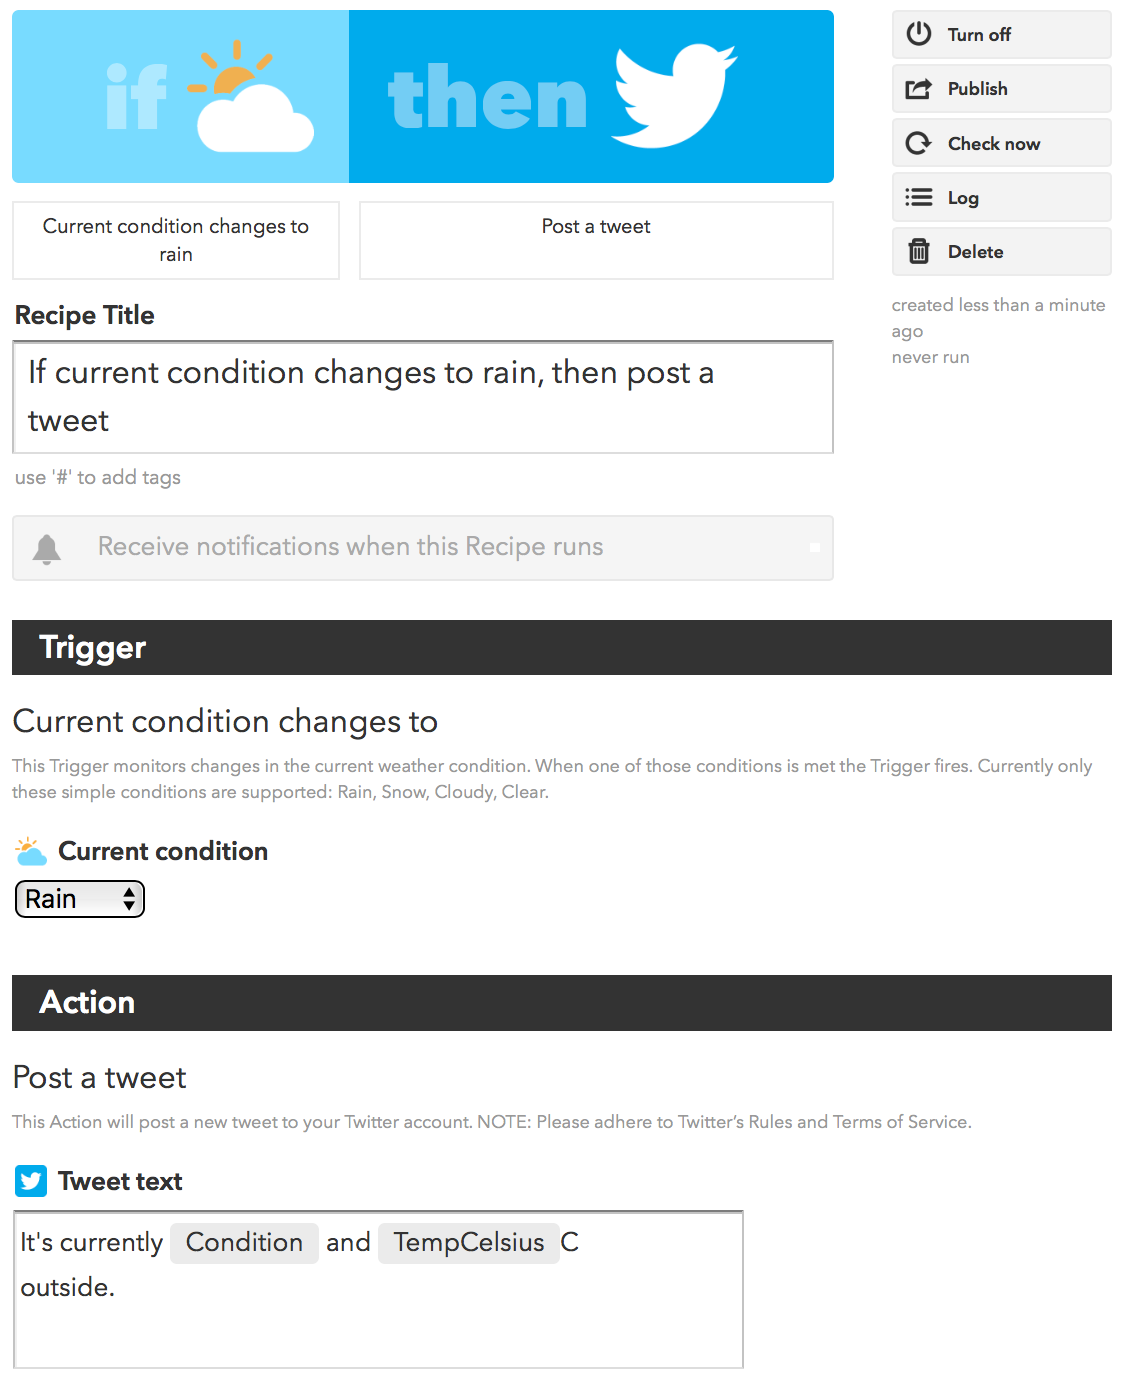
\includegraphics[width=0.7\textwidth]{images/c4/IFTTT.png}
\caption{An example of a workflow created using \ac{IFTTT}: when the condition in the user's location changes to rain (trigger) it will automatically post a tweet (action).}\label{fig:ifttt}
\end{figure}

During the first phase --- lasting 30 minutes --- participants were instructed in the context of this research and the problem it is addressing by the facilitator. They were shown some videos outlining the process of developing workflows on \acr{IFTTT}~\cite{IFTTT}, a widely popular \ac{EUD} Web mashup system~\cite{Malizia:2011tw}; it allows users to create simple event-based \emph{if-then}-style workflows with different Web services and acts as a hub connecting their events' triggers with actions: one can describe simple rules by selecting the event that will trigger the workflow (e.g., when the current temperature rises above a certain value or when the user edits a specific file on Dropbox) and an action that should be performed by any other --- even the same --- supported Web service (e.g., tweet about it or send the file via email), as shown in figure~\ref{fig:ifttt}. This platform is very flexible and can be easily integrated into most people day-to-day activities on the Web to support them. Thus, it was chosen to showcase different types of simple workflows, their inner logic and how the trigger selection provides the subsequent action with anchors dependent on the output's type: for instance, when the event concerns a location the action can access its GPS coordinates, when it involves a text file the action will be able to use its content, and so on.

Then participants were shown a video of an existing \ac{TUI} system --- the Tangible 3D Tabletop~\cite{Dalsgaard:2014ut} --- which summarized the benefits of this interaction paradigm. In particular, two different ways of employing tangible objects in educational systems were shown~\cite{Zuckerman:2005:ETI:1054972.1055093}, in order to prompt them to produce different ideas: \acp{FiM} are building blocks used to design and represent real-world things, objects, and physical structures, for example, 3D building blocks to represent buildings on a map (figure~\ref{fig:tangible:a}). \acp{MiM} are building blocks focused on modelling more conceptual and abstract structures, for instance, tangibles used to control RGB colour blending (figure~\ref{fig:tangible:b}).

\begin{figure}[ht!] 
  \begin{subfigure}[b]{0.48\linewidth}
    \centering
    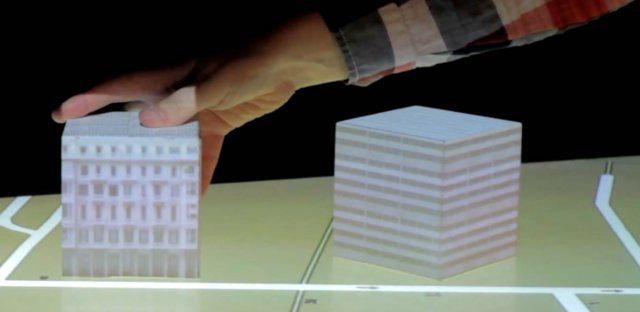
\includegraphics[width=0.75\linewidth]{images/c4/BuildingTangible.jpg} 
    \caption{3D building fa\c{c}ades on tangibles placed on a map.}\label{fig:tangible:a}
    \vspace{6ex}
  \end{subfigure}
  \begin{subfigure}[b]{0.48\linewidth}
    \centering
    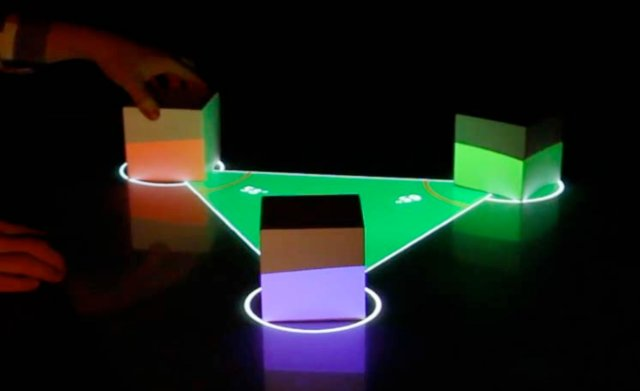
\includegraphics[width=0.75\linewidth]{images/c4/RGBTangible.jpg} 
    \caption{Three tangibles used as RGB colour blenders. The base colour is projected onto each tangible, and users can change the hue of the triangle drawn within the tangibles by turning them.}\label{fig:tangible:b}
  \end{subfigure}
  \caption{Two examples of different metaphors involved in the Tangible 3D Tabletop system~\cite{Dalsgaard:2014ut}.}\label{fig:tangible}
\end{figure}

After the introduction, participants started a 30-minute discussion about ideas and challenges for the design, focusing on an \ac{IL} scenario involving users with no previous programming experience. The gathered feedback is summarised in the following.

\subsubsection{Study Findings}
The features suggested by participants were clustered by subject --- concerning either the system's tangible objects or its digital syntax. Here are the main findings from the focus group:

\paragraph{Tangible features} Participants remarked the fact that the system should react only upon user actions and provide useful feedback through a specific communication channel, in agreement with one of the main principles of \acp{NUI}~\cite{Wigdor:2011bi}. Many suggestions focused on the preferred channel to be used to provide feedback. These included providing tangible objects with a touch-sensitive mechanism in order to activate the feedback only when users physically touch objects on the table, in order to highlight whether selected objects are compatible with each other (fulfilling the workflow constraints). Moreover, the feedback communication channel of choice can be a physical one as well: a magnetic attraction between objects could indicate whether two workflow's components are compatible with each other, while repulsion might represent the opposite. An\-oth\-er par\-tic\-i\-pant sug\-gest\-ed employing haptic feedback built into the tangibles to communicate compatibility between different ones.

\paragraph{Digital features} Another set of suggestions were directed towards the digital representation of the platform's syntax. First, the blocks' digital representation should help users understand components' constraints by using, respectively, different and similar colours or shapes for incompatible and compatible components. Also, since a workflow's composition is usually performed one component at a time, i.e.\ by selecting a function that will follow the latest assembled one, the system shall aid users on the next available components to be chosen by changing the colour or the shape of the currently assembled workflow. Lastly, available components should be displayed all at once, giving users an overall view of the system's capabilities. However, this can also increase mistakes. Since the target group is inexperienced users, the system should assist them in finding the right way of assembling different components, when they cannot figure it out themselves; a useful suggestion on this regard is to provide some sort of ``translation tool'', which --- once a user selects two blocks incompatible with each other --- shows them at least one possible way of choosing other components in between to connect the two blocks, assisting users during the composition phase.

The suggestions stemming from the workshop drove a preliminary design of the system, whose details are presented in the next section.

\subsection{Preliminary Design}\label{sec:pdesign}
The system design aims to provide users with a platform that can be employed in a variety of \ac{IL} domains --- e.g., in museums or workplaces --- to cultivate \ac{CT} skills through objects manipulation.

The platform is deployed on tabletop displays, which naturally foster collaboration as required in \ac{IL} domains, and consists in a Block-based Programming environment~\cite{Mohamad:2011kz} to support inductive processes --- widely used in systems like Scratch~\cite{Resnick:2009bd} and Blockly~\cite{BLOCKLY} --- that has proven to have a low learning threshold for non-programmers, as thoroughly discussed in the previous chapter.

It allows users to create, share, modify and reuse simple workflows, namely sequential processes combining different services in a data-flow fashion, where the output of a service becomes the input of the following one, integrating into users' daily routine while supporting \ac{IL} through inductive processes. 

Users impart instructions through a visual syntactic construct in a \ac{PbI} fashion rather than by demonstrating their intentions to the system: indeed, making a workflow's inner architecture transparent to users can help them to better understand its sequential logic and behaviour, providing further design opportunities to improve their \ac{CT} skills and easily integrate the system into rather different scenarios.

The system's blocks correspond to workflow components (i.e.\ functions) that can be assembled together as in many other Block-based Programming environments; each block receives specific formats of data as input and produces different ones as output based on its inner workings and its location within a workflow's logic. Type constraints on different blocks inputs and outputs are afforded using different shapes, as in a puzzle.

A tangible object is associated with the main block --- a circle halo with a single hollow to accommodate the next piece to be added to the workflow --- which will move alongside the object on the main display's surface; moving the main piece towards another will add the latter's related function to the workflow --- only if the two shapes are matching, that is to say, the latest output is compatible with the required input (figure~\ref{fig:walkthrough:a}). This mechanism aids end-users in understanding the data-flow approach as well as type constraints.

Inputs requested by services might be quite heterogeneous and complex depending on the scenario, requiring at this point a precise and familiar input mechanism that can adapt to different needs. Hence, smartphones have been se\-lect\-ed as the tan\-gi\-bles controlling the main blocks in the system: they represent objects whose movements allow users to interact with the system, i.e.\ they form the physical and digital representation of information in the system, and are already equipped with all the sensors and feedback mechanisms needed to implement the designers' suggestions obtained from the focus group and push the interaction even further. They can be used to adapt the system to the different users' preferences since they hold much of their personal information. Moreover, they can be used to display a wide range of widgets that can be presented to end-users depending on the specific service being accessed (e.g., a virtual keyboard for text input).

\begin{figure}[ht!]
\centering
\includegraphics[width=0.7\textwidth,trim={800 100 0 100},clip]{images/c4/protopic.png}
\caption{An example of a workflow being assembled using the proposed system: a keyboard widget is displayed on the smartphone once a new piece requiring an input is assembled.}\label{fig:proto}
\end{figure}

Widgets vary depending on the type of input requested: selecting a single option among several will prompt the user with a list box, a single action to be performed will display a button, and a generally unstructured raw text to be inserted will present a keyboard (figure~\ref{fig:proto} and~\ref{fig:walkthrough:b}). Once a user enters the requested input on a widget, the latter disappears from the smartphone and the projected halo surrounding it opens up a new hollow to allow for the next block to be inserted (figure~\ref{fig:walkthrough:c}); then using the input, only the hollow that is compatible with it is displayed, preventing invalid compositions. When a workflow is completed, it can be run by pressing a button on the smartphone (figure~\ref{fig:walkthrough:d}).

\begin{figure}[ht!] 
  \begin{subfigure}[b]{0.48\linewidth}
    \centering
    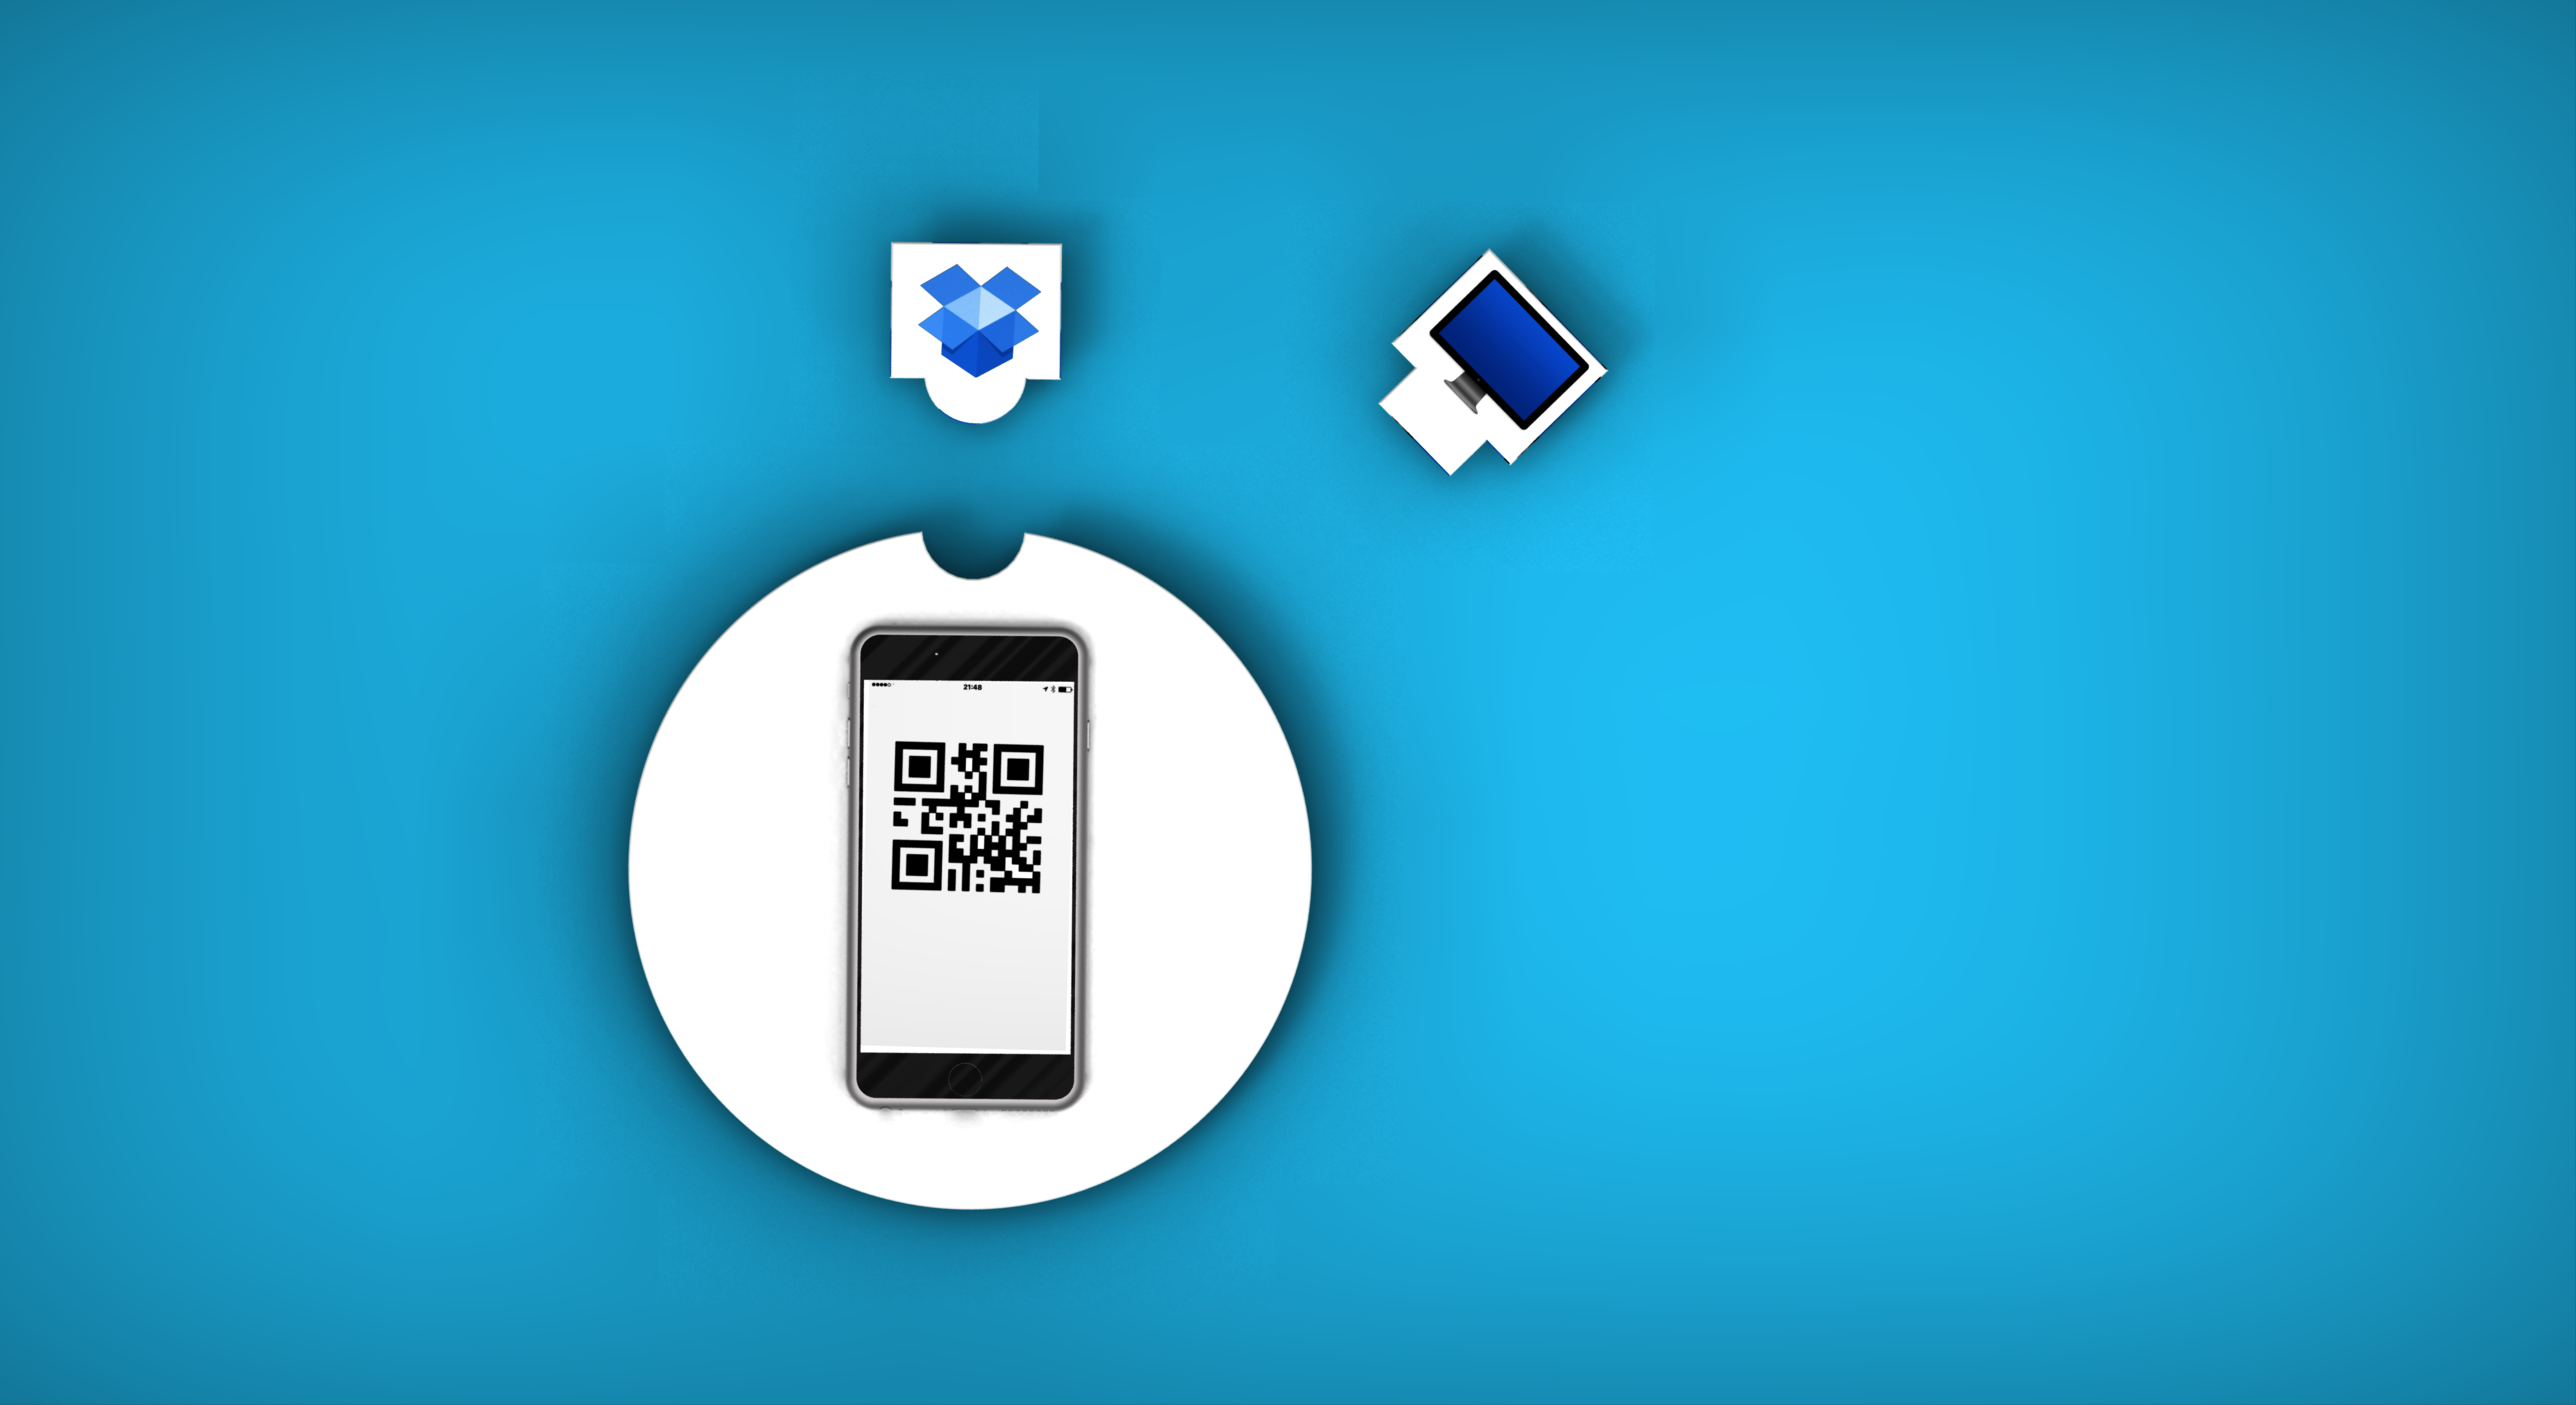
\includegraphics[width=0.75\linewidth,trim={800 200 1600 200},clip]{images/c4/TAPAS-1.png} 
    \caption{The first piece is se\-lect\-ed and add\-ed to the cur\-rent work\-flow by mov\-ing the smart\-phone to\-wards it.}\label{fig:walkthrough:a}
  \end{subfigure}\hfill
  \begin{subfigure}[b]{0.48\linewidth}
    \centering
    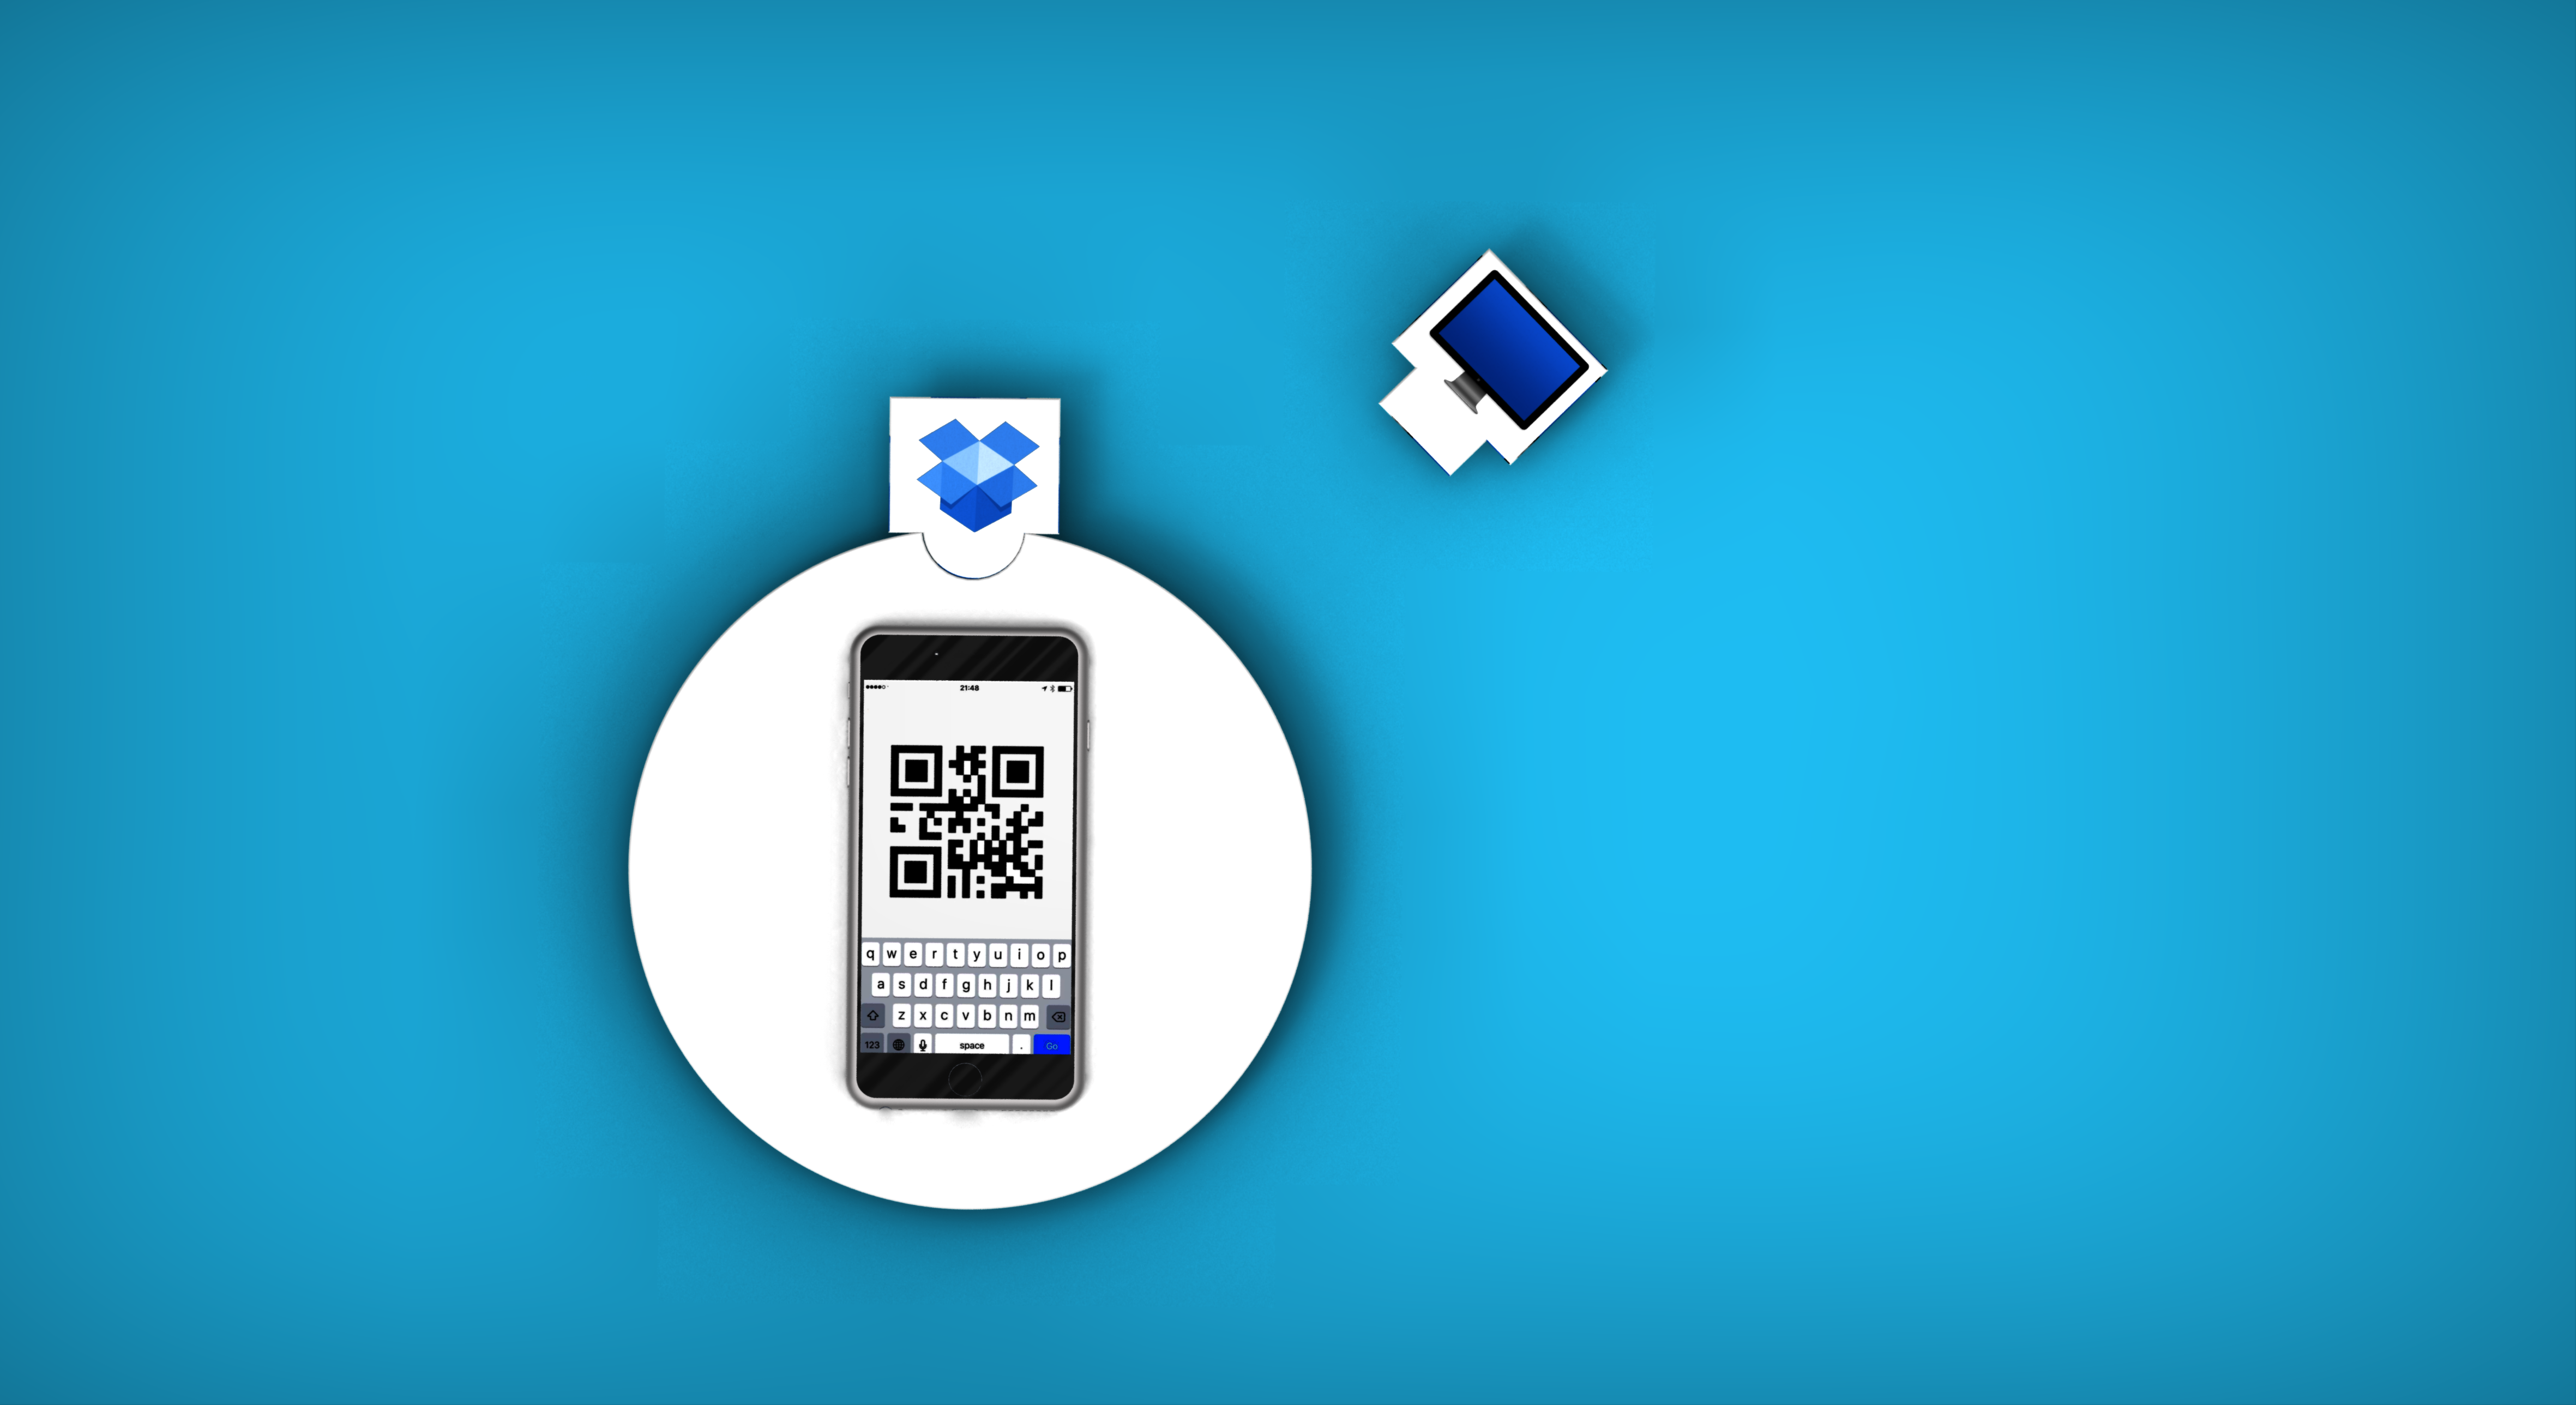
\includegraphics[width=0.75\linewidth,trim={800 200 1600 200},clip]{images/c4/TAPAS-2.png} 
    \caption{The cor\-re\-spond\-ing widg\-et is dis\-played on the smart\-phone wait\-ing for us\-er in\-put.}\label{fig:walkthrough:b}
  \end{subfigure}
  \begin{subfigure}[b]{0.48\linewidth}
    \centering
    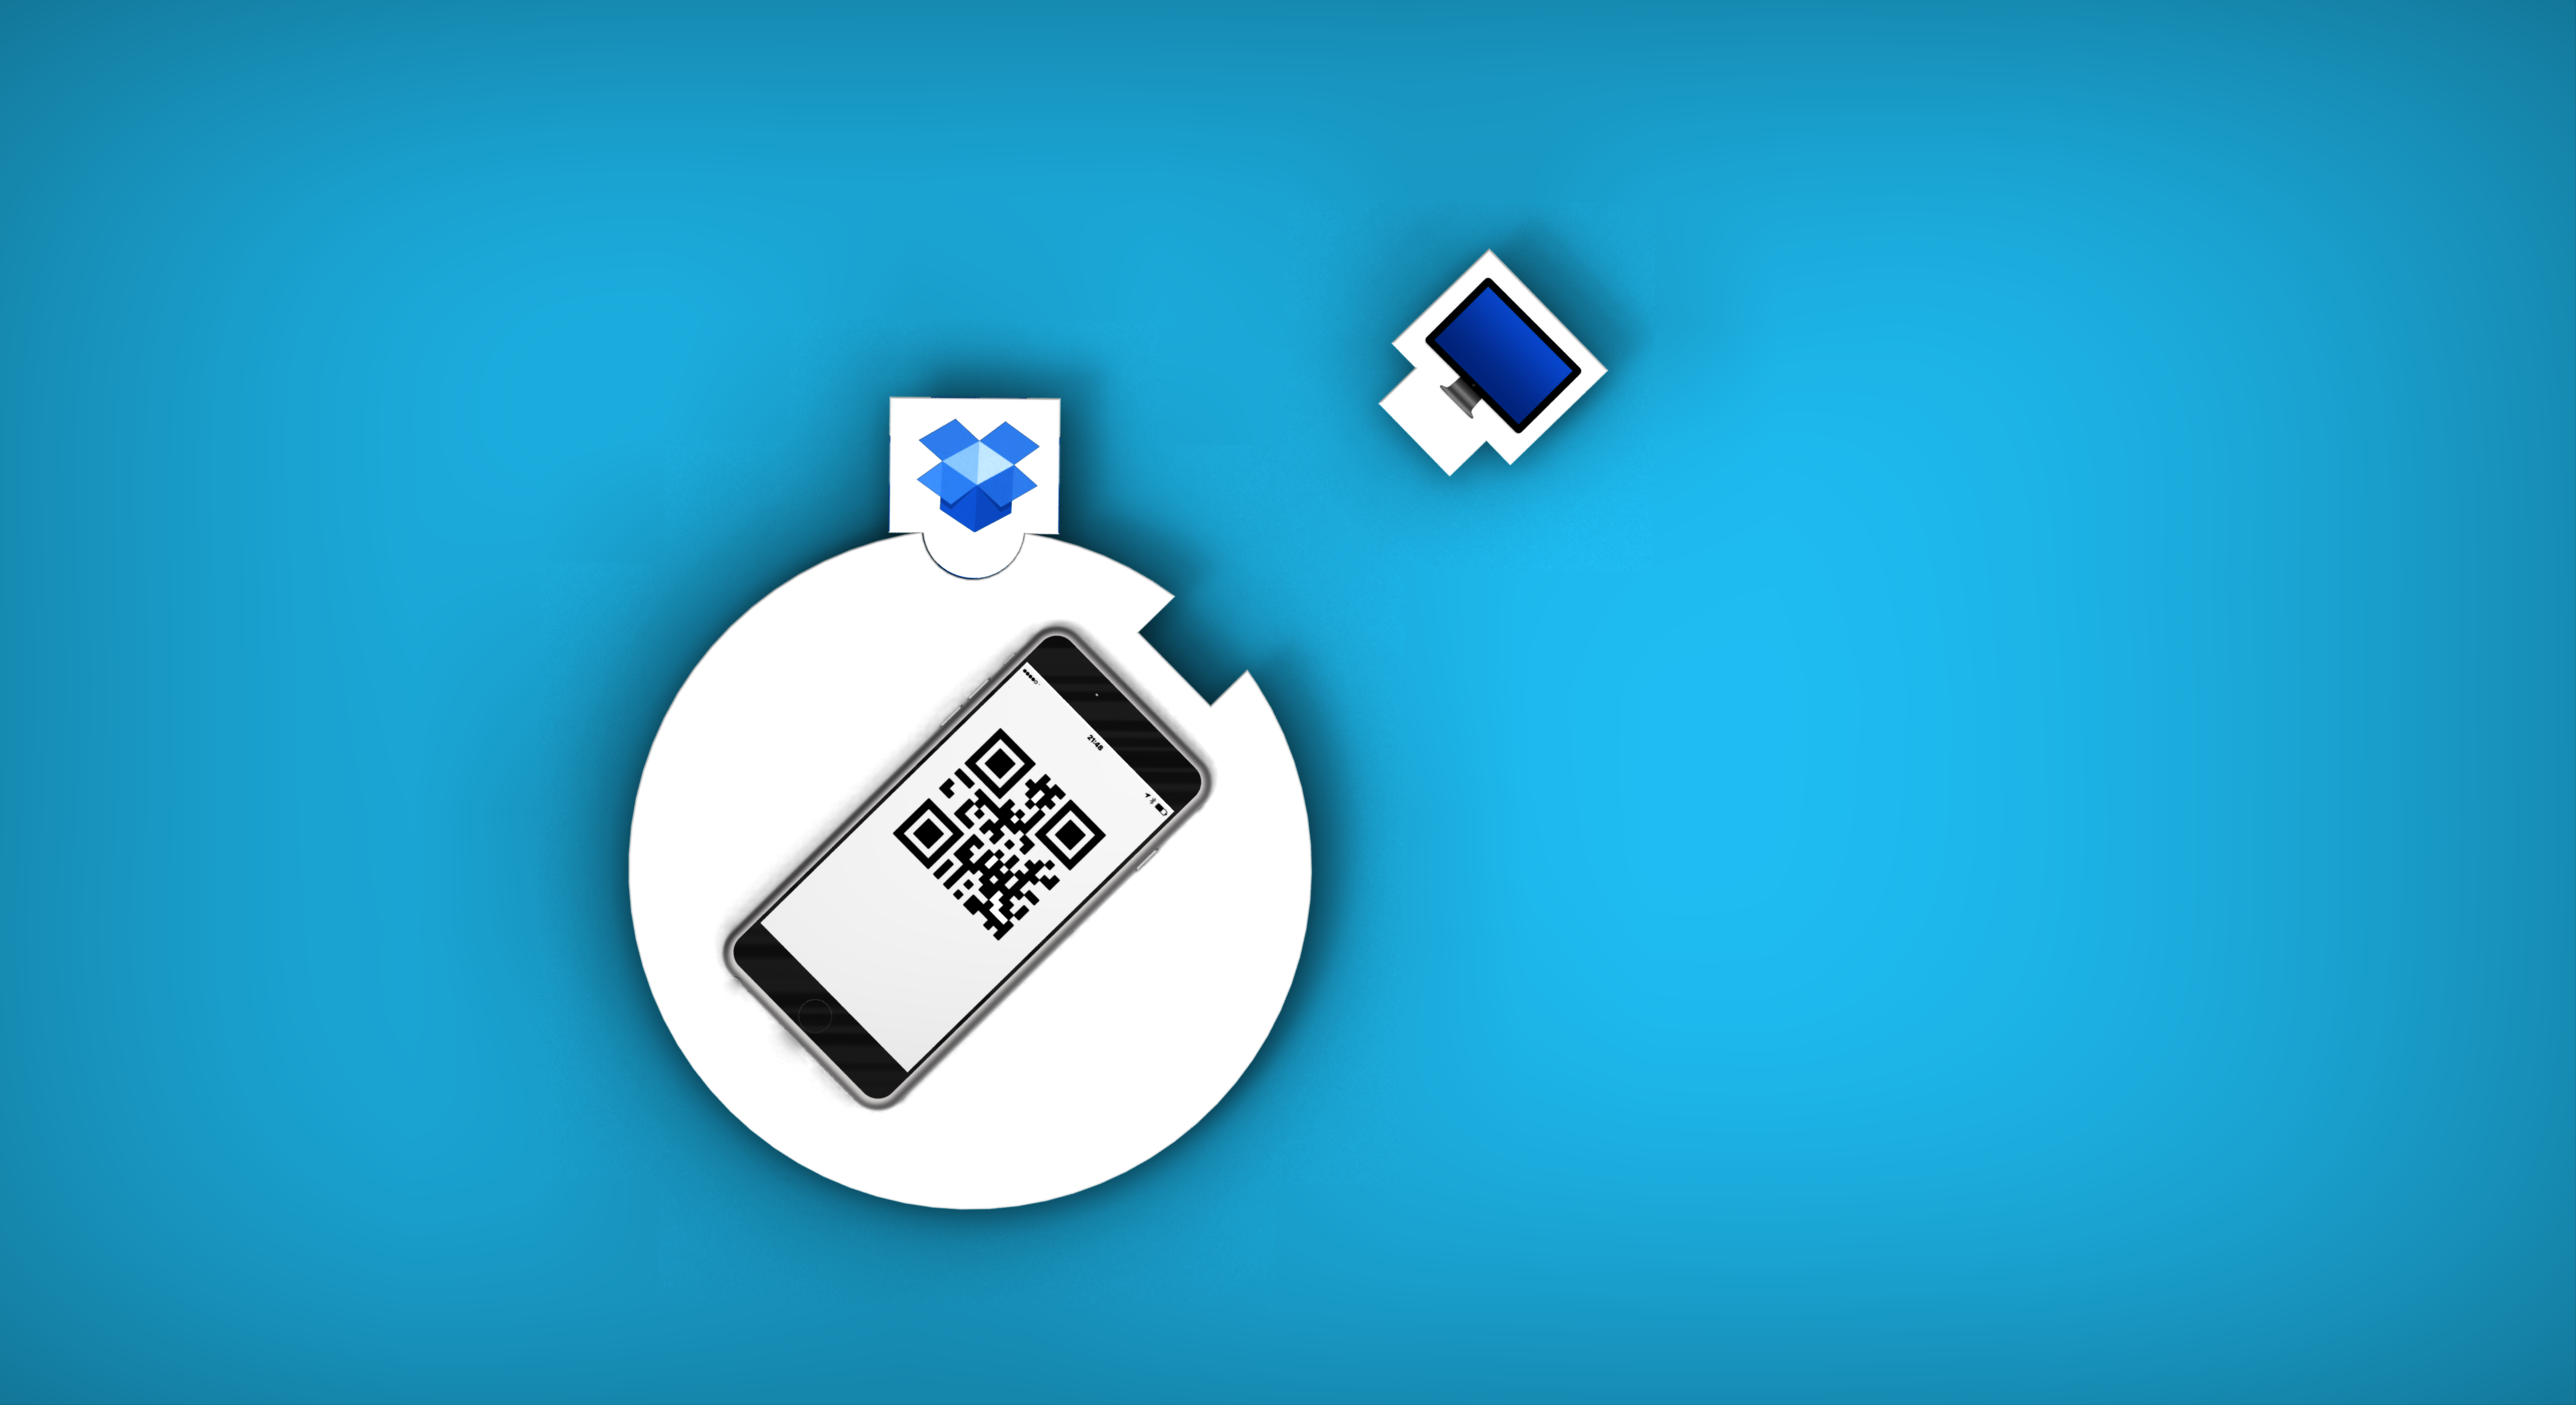
\includegraphics[width=0.75\linewidth,trim={800 200 1600 200},clip]{images/c4/TAPAS-3.png} 
    \caption{Once the in\-put is in\-sert\-ed, a piece whose in\-put match\-es the cur\-rent work\-flow's out\-put can be add\-ed.}\label{fig:walkthrough:c}
  \end{subfigure}\hfill
  \begin{subfigure}[b]{0.48\linewidth}
    \centering
    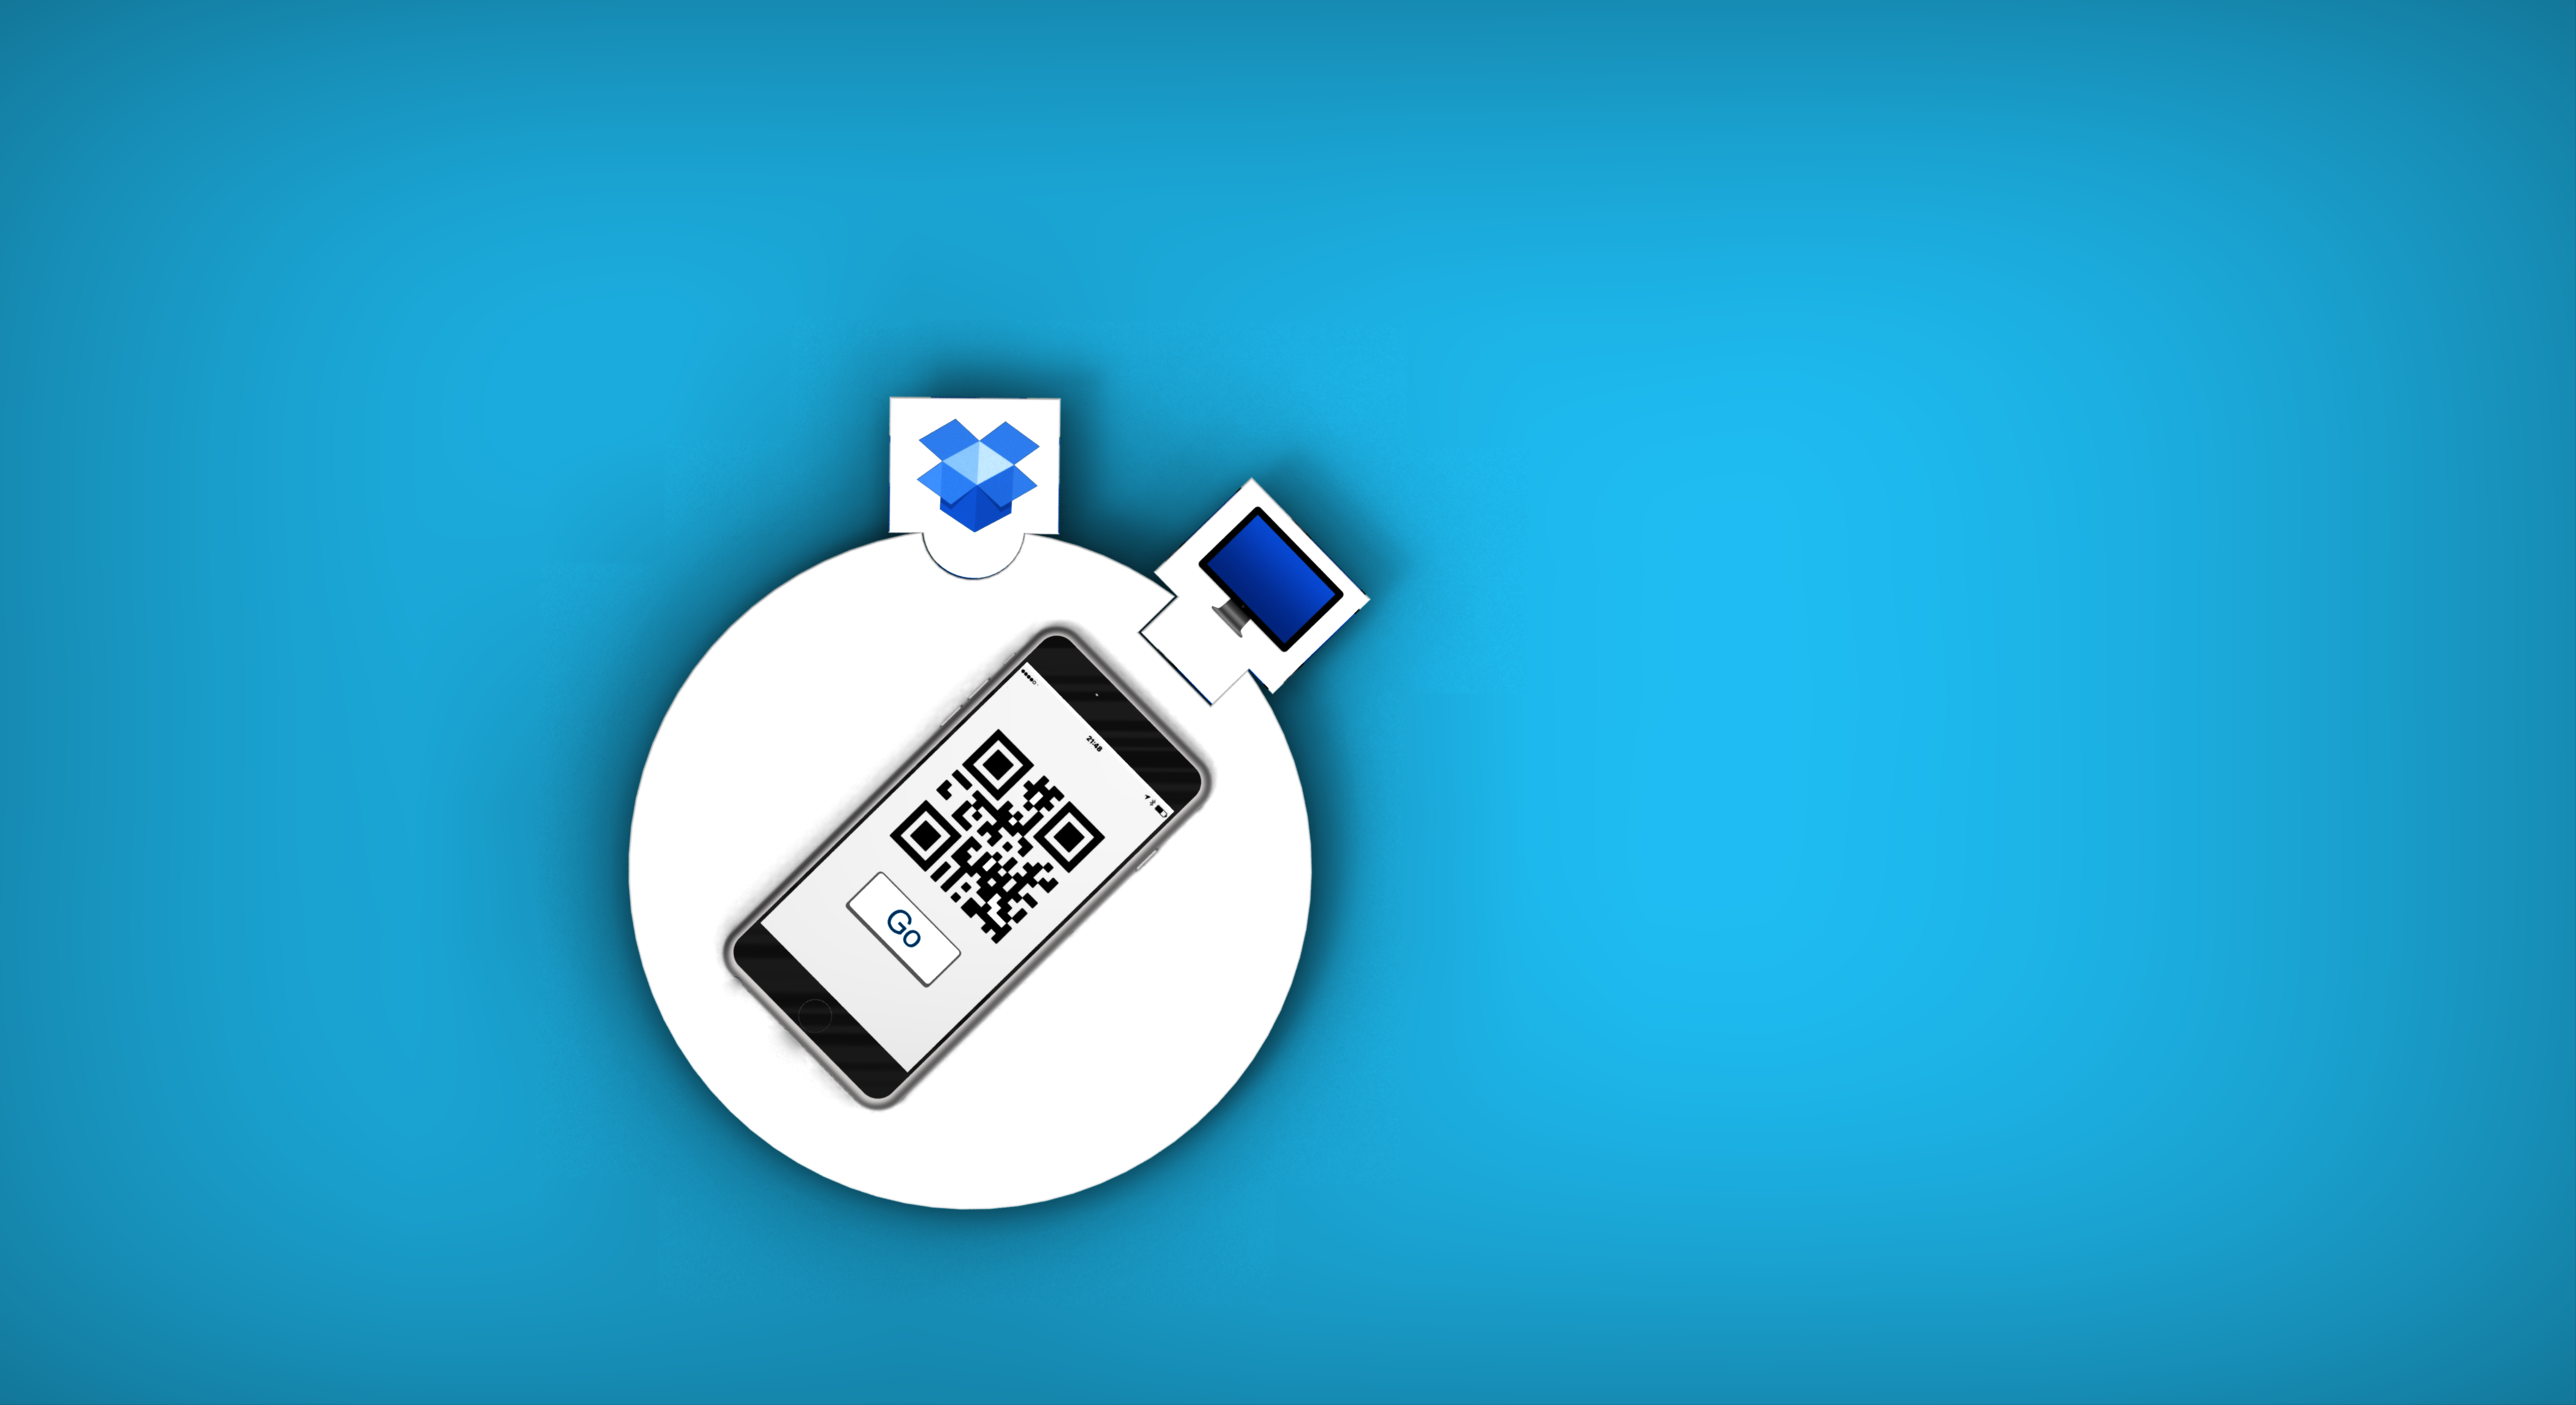
\includegraphics[width=0.75\linewidth,trim={800 200 1600 200},clip]{images/c4/TAPAS-4.png} 
    \caption{Fi\-nal\-ly, the work\-flow is com\-plet\-ed and the us\-er can run it from her smart\-phone.}\label{fig:walkthrough:d}
  \end{subfigure}
  \caption{A step-by-step walkthrough of building a workflow.}\label{fig:walkthrough}
\end{figure}

The next section reports a study carried out to evaluate the platform and address the Research Question formulated in the introduction of this chapter related to the effects of physical manipulation on the development of \ac{CT} skills in \ac{IL} domains.

\section{Evaluation}\label{sec:ev4}
This section presents the goals, hypotheses, and description of the experiment carried out to test the designed system, following the guidelines of the American Psychological Association~\cite{Wohlin:2000:ESE:330775}.

\subsection{Goals}
The goal of the experiment is to evaluate the system design and tangible-based interaction paradigm in a real-world \ac{IL} scenario, namely a work project meeting. The purpose is to evaluate whether this system might be employed in a given \ac{IL} scenario and investigate the effects of \ac{TUI} on the development of \ac{CT} skills.

\subsection{Research Question}
\ac{CT} is a set of skills that can help people  play a more active role in their day to day life, due to the massive impact of software in today's Information Society. Nonetheless, people struggle in dealing with the abstract concepts underlying it, thus it is important to support them in fostering such skills with new and engaging ways without getting in between their actual routine. Constructivist theories suggest that objects manipulation --- underpinning \acp{TUI} --- might be an effective way of aiding end-users in making such highly abstract concepts more tangible and understandable.

Supporting users in developing \ac{CT} skills is even more important in \ac{IL} scenarios, where learning is predominantly unstructured, experiential, and noninstitutional, making the experience self-directed and personalised with higher motivations and efficacy. 

Promoting \ac{CT} skills in \ac{IL} domains through physical objects manipulation might help to lower the barriers of \ac{CT} by integrating learning in their daily routines and supporting users in dealing with such abstract concepts through their day-to-day experiences.

The proposed system has been developed with the aim of investigating the influence of \acp{TUI} on \ac{CT} skills in multiple \ac{IL} scenarios. It employs a tangible-based interaction with a tabletop surface --- naturally fostering collaboration --- and supports inductive processes by means of assembling workflows to solve simple tasks. Thus, it has been designed to easily integrate into users' day-to-day routine to support \ac{CT} skills.

The main research question addressed by the evaluation is then \textit{``Can physical objects manipulation help foster \ac{CT} skills in \ac{IL} domains?''}.

\subsection{Experiment Design}
Due to the openness of the range of scenarios analysed --- i.e.\ \ac{IL} scenarios --- an exploratory research design was used, comprising two phases:
\begin{enumerate}
  \item a combination of oral feedback and observations of end-users engaging with the prototype in a semi in-the-wild scenario, i.e.\ taking place in a real-world setting and addressing real-world problems, as a way of testing it in a generic \ac{IL} environment, and
  \item semi-structured interviews of domain experts, in order to gather more generic and less domain-specific feedback.
\end{enumerate}

\subsection{Participants}
\subsubsection{First Phase}
The study involved end-users selected among Brunel University second-year students in the Department of Computer Science, College of Engineering and Design. As part of their degree they are clustered into groups of 4-6 and tasked with an Android application development project to be undertaken during the course of the year; they are required to meet and work collaboratively every week, normally in the library or in one of the college's meetings rooms, and can use a range of available tools to work together and share information with each other (online dedicated forums or drives, laboratory spaces with coding facilities, etc.). The development is supervised by a teaching staff member, whom they usually meet all together as a group once a week. The objective of these meetings is not to develop the Android application --- which is an individual task --- but to coordinate and organize a project plan, eventually designing a Gantt diagram to split the workload into individual tasks. This is a time when students self-direct their activities, exchange suggestions, and support each other, being a proper example of a real-world \ac{IL} scenario.

In particular, three groups of students in their second year participated to the study, made up respectively of four (1 female, 3 males), five (1 female, 4 males), and six (all males) students, reflecting the real project activity requirements and average group size; participants had no prior knowledge of the system, but attended their introductory programming course during their first year, thus they already had some programming and problem-solving experience.

\subsubsection{Second Phase}
Three interaction design experts were involved to get feedback on the featured modality; they were composed of two HCI experts --- with a mixture of academic and industry backgrounds --- and a product designer, all with more than 20 years of experience in their fields. By involving more experienced participants, the proposed interaction modality has been further evaluated through a less domain-specific point of view, considering a wide range of \ac{IL} domains for its application.

\subsection{Settings and Procedure}
\subsubsection{First Phase}
The study took place within the University facilities, in a room inside the Department of Computer Science designated to students and staff meetings, where many public interactive displays are already being deployed and used with a researcher present. It was conducted in three different sessions, one for each group of students, lasting half an hour each, and was a preliminary evaluation of the system's feature set and interaction modality.

Due to the inexperience of participants for this phase, eliciting the discussion around the system interaction modality might not have been easily gathered employing only a paper and pencil approach. Thus, students were prompted with it as a ``provotype'' --- i.e.\ a provocative prototype, namely a prototype that deliberately challenges stakeholders' conceptions by reifying and exposing tensions of existing practice in a context of interest~\cite{Boer:2012ku}; this includes a small set of features highly tailored to the evaluation scenario (i.e.\ university students collaborating with each other).

The features made available to participants, each rendered with a different block, were:
\begin{enumerate*}[label={(\arabic*)}]
  \item selecting and downloading a file from the user's Dropbox account;
  \item displaying a downloaded PDF file or an image on the main tabletop screen;
  \item searching for a book in the university library and retrieving its location inside the building depicted in an image; and
  \item sending a text document to a specified email address.
\end{enumerate*}

For instance, one could pick 1 and 2 (in this order) and the composed application would download a PDF from the user's Dropbox folder and display its content on the big screen (as depicted in figure~\ref{fig:walkthrough}); composing 3 and 2 together would result in looking for an available book in the university library and displaying its location on the big screen.

\begin{figure}[ht!]
\centering
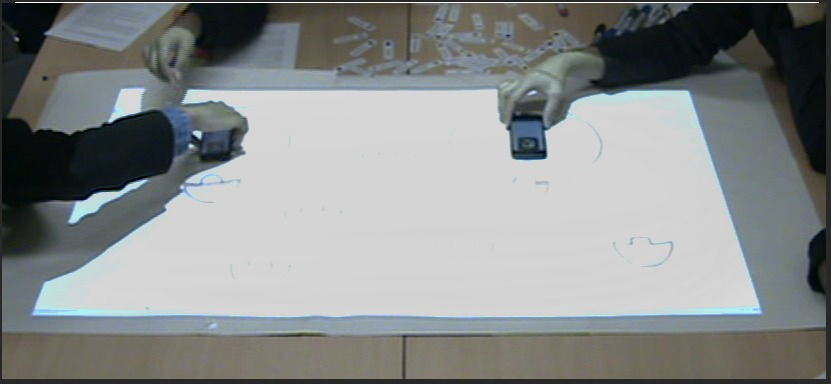
\includegraphics[width=0.7\textwidth]{images/c4/studs.png}
\caption{One of the participating groups to the study.}\label{fig:studs}
\end{figure}

Each session lasted 30 minutes and started by briefly introducing the current version of the system to participants, explaining to them how the system works. They were then left to play with it for 15 minutes (figure~\ref{fig:studs}), and finally, a semi-structured interview was carried out, mainly focused on the proposed interaction modality.

\subsubsection{Second Phase}
Semi-structured interviews were carried out in a controlled environment (figure~\ref{fig:des}), namely during a workshop on the island of Tiree, during the bi-annual Tiree Tech Wave, a gathering of experts in various fields, ranging from interaction designers and artists to computer scientists.

\begin{figure}[ht!]
\centering
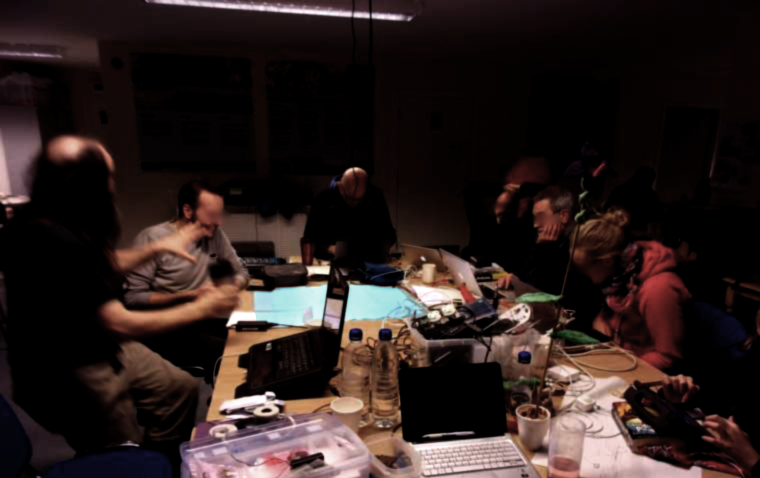
\includegraphics[width=0.7\textwidth]{images/c4/tiree.png}
\caption{The designer study setting.}\label{fig:des}
\end{figure}

Individual sessions lasted 45 minutes, starting by introducing the prototype, explaining the rationale behind its design and the targeted scenarios; it was then followed by a brief demonstration of how it works, going through some examples of its usage in real-world \ac{IL} scenarios. Finally, a semi-structured interview was carried out focusing on the strengths and weaknesses of the prototype in relation to the interaction modality and its applicability in \ac{IL} domains to foster \ac{CT} skills, more precisely covering the easiness of the puzzle metaphor, the use of smartphones as tangible objects, future application scenarios, and missing features.

\subsection{Summary}
\added[comment={MP3, MP8, D18}]{To recap, table \ref{tab:ch4summary} presents a summary of the specific \ac{CT} dimensions as defined in~\cite{Brennan:2012} examined in the evaluation, along with the related assessment approach, as reported in chapter \ref{chap:background}.}

\begin{table}[ht!]
  \caption{Summary of the specific \ac{CT} dimensions~\cite{Brennan:2012} considered by the evaluation with the related assessment approach.}\label{tab:ch4summary}
  \centering
  \begin{tabular}{M{0.2\linewidth}m{0.5\linewidth}M{0.2\linewidth}}
    \toprule
    \textit{\ac{CT} Dimension} & \textit{Description} & \textit{Assessment} \\
    \midrule
    Concept: sequences & Ex\-press\-ing a par\-tic\-u\-lar ac\-tiv\-i\-ty or task as a se\-ries of in\-di\-vid\-u\-al steps or in\-struc\-tions that can be ex\-e\-cut\-ed by the com\-put\-er. & Project Analysis (First Phase Provotype) \\
    Practice: abstracting and modularizing & Building something large by putting together collections of smaller parts. & Artefact-Based Interviews (First Phase Interviews) \\
    \bottomrule
  \end{tabular}
\end{table}

\added{Moreover, the second phase of this evaluation preliminarily investigated over the interaction modality of \ac{TAPAS}.}

\section{Results}
Data collected in both phases were analysed by performing a content analysis on the gathered feedback and observations.

\subsection{First Phase}
Overall results point out how the proposed user experience was considered quite satisfactory by participants; as expected, students' feedback mostly focused on missing features and the interaction with the system.

Each group managed to successfully assemble (at least once) two workflows while they were playing with it: the first one started with downloading a PDF file from a Dropbox account and displaying a preview on the main tabletop surface, while the second one started with looking for a specific book in the university library and depicting its location on the main screen.\deleted[comment={D19}]{ One group even assembled a more complex workflow, consisting of downloading a text file from Dropbox and sending it via email to an address of choice.}

From the gathered feedback it seems that a \ac{TUI} is an easy and effective way of interacting with the system throughout the composition of a workflow. Even though all participants are \ac{CS} undergraduates, their second-year group project is their first chance of tackling a wider problem-solving scenario, unlike their first year's individual development of smaller applications. This more complex project requires them to learn abstraction and decomposition skills, whilst collaborating with peers. Using the puzzle metaphor and workflows together with tangible interaction \replaced{helped}{seemed to help} them build the required \ac{CT} skills: for instance, collaboratively planning and designing the application's tasks and assigning them to each participant \replaced[comment={D20}]{could be}{seems like} a suitable scenario to practice abstraction and composition skills. Moreover, as with API development, the recipe metaphor provides different levels of transparency and abstractions useful to generalize the problem, whilst assembling blocks might help with decomposing a bigger problem into smaller ones~\cite{Wing:2008cv}.

Nonetheless, the feedback showed that just a tangible interaction doesn't seem ``natural'' when it comes to manipulating outputs: every participant trying out the prototype attempted to move images displayed on the screen with their fingers, suggesting that manipulating items through objects might feel ``natural'' only when operating in composition/developing mode and there is a perfect mapping between the physical and the digital object, but not when there is actual content the user needs to directly manipulate available on the screen. This \replaced{might be a result}{follows directly from the choice} of employing a \ac{PbI} paradigm\added[comment={D21}]{ to be able to repurpose the system to different domains}, which uses a syntactic construct to specify a workflow's instructions as opposed to exploiting only contextual actions on resulting artefacts --- i.e.\ \ac{PbD}.

From the interaction point of view an interesting remark was made by one of the participants: continuously tracking the smartphone's position on the surface using a fiducial marker requires users not to cover its display with their hands when moving it; however, the hand position on the smartphone might depend on the posture: if a user is standing, he/she might feel more ``natural'' to hold it from above --- thus covering the fiducial marker with the palm --- while a seated user might feel more comfortable grabbing it from the side, without covering its display, allowing for its movements to be tracked. Because the majority of existing smartphones are shaped in the same way, it might be worth studying this ergonomic effect in more detail, in order to establish whether users could be provided with a physical enclosure affording the ``right'' way of holding the smartphone or whether it is a negligible effect when the system runs on horizontal displays placed at a certain distance from the floor.

The same users appear to cope easily with the proposed interaction modality during the workflow editing phase, but a different interaction style has to be devised when it comes to manipulating results.

\subsection{Second Phase}
Designers liked the overall idea and the personalization approach for different scenarios, namely using a smartphone as a tangible instead of just a passive object to identify users and link their personal information with the movements they perform on the very same device. In particular, they liked the way blocks use shapes to establish type constraints as it looks like a straightforward way of understanding the composition of workflows to address users' needs.

They recognized the potential of such a system in public spaces, due to its ease of deployment and the cheapness and high availability of the technologies involved: thanks to the simple architecture, it allows deployment in any digitally augmented surface just by installing an RGB camera and running the application on a production server; it can be left in public spaces for a long period of time without the need to perform mundane maintenance operations aimed at adding new features, since users can repurpose it themselves.

Some of their suggestions focused on the way data are presented to users and the use of the dynamic widget to get some input from them: due to the kind of data handled right now --- namely lists of files within directories or book titles in a database --- it makes sense to prompt users with a choice from a list or offer a keyboard to input raw text. Nevertheless, this will not be the case when dealing with more structured data types, such as points of interest on a map: therefore, they suggested that due to the complexity of workflows that might be put together by end-users, widgets might be designed to be more flexible and personalizable depending on the two-fold level of interaction between the user perspective and data perspective related to the specific data handled by the widget. They emphasized that the two perspectives are interlinked and reinforced mutually. Elements of human-centred information visualization have to be considered in the redesign of the widgets for the next interaction prototype; for instance, by following visual metaphors that incorporate semantic relationships of visual objects both in the physical (tangible) and virtual (digital) world~\cite{Majumder:2013wt,Bigelow:2014th}.

Furthermore, interviewees pointed out how the continuous back and forth between interacting with the smartphone to input data and with the large display to assemble workflows might be confusing for users: interacting with two different devices, each one with a different interaction style --- i.e.\ tangible on the tabletop, multi-touch on the smartphone --- and different underlying metaphors, requires a relatively high cognitive effort in constantly switching paradigm and some users might also miss what is happening on one device while they are too focused on interacting with the other. That is why interviewees suggested keeping the tabletop as the main interaction focus by providing a mixed interaction modality: moving the smartphone will still be used to assemble the puzzle pieces but once one of them requires a certain input, the widget will appear close to it on the tabletop surface and users will interact with it using their fingers.

The final observation concerns the blocks shapes: although it appears to be quite an easy to grasp concept, its efficacy might be improved by offering some additional visual cues; interviewees suggested that in addition to shapes to indicate functions compatible with the currently generated output, it might highlight the available ones and darken the incompatible ones, even when the former is not available due to network outages or other problems, or even associate colours to shapes.

To recap, there are positive elements in the system design for \ac{EUD} of workflows to be employed in many existing \ac{IL} scenarios\added[comment={D22}]{ to foster \ac{CT} skills}, such as the Block-based Programming paradigm, the use of the smartphone as being tangible and personal, and the ease of prototype deployment in-the-wild due to its low-cost and flexible architecture. Nonetheless, there are some challenges to be addressed in the future in terms of interaction design requirements, such as the flexibility of widgets and improving the visual cues to highlight available functionalities\added{, which might hamper the usability and get in the way of the learning experience}.

\section{TAngible Programmable Augmented Surface}\label{sec:tapas}
The results of the evaluation phase highlighted the validity of employing the developed platform in \ac{IL} scenarios and prompted for its extension to make it easily repurposable to different domains and include some of the gathered feedback.

In the following, the \ac{TAPAS} architecture is presented, developed to investigate the influence of \acp{TUI} on \ac{CT} skills in different \ac{IL} scenarios.\deleted[comment={D23}]{ The aim of the prototype is to integrate into end-users' day-to-day routing by allowing them to solve simple tasks while fostering their \ac{CT} skills.}

\subsection{Architecture}\label{sec:tapasarch}
\acs{TAPAS} comprises a horizontal tabletop display and an RGB camera capturing the movements of the users' smartphones on the main display's surface using fiducial markers~\cite{chilitags} (i.e.\ images used as a point of reference when placed in the camera's field of view), as summarized in figure~\ref{fig:arch}; it supports --- and later extends --- the \ac{TUIO} protocol~\cite{kaltenbrunner2005tuio}, already adopted by many research communities within the \ac{TUI} area as a general and versatile communication interface between tangible tabletop controller interfaces and underlying application layers, which has been designed specifically for interactive multi-touch tabletop surfaces.

When a user logs into the provided Web application running on a smartphone using her credentials, this will display a fiducial uniquely assigned to that account. The system can then track the position of the fiducial across the tabletop surface, knowing to whom it belongs.

Tracking objects using fiducials allows supporting physical object other than smartphones, each providing its own set of sensors and feedback mechanisms if any. The \ac{TUIO} protocol, however, is quite generic and limited to tracking positions of generic objects in a 2D space, without providing a way for objects to expose their supported I/O interfaces. For this reason, an extension of the \ac{TUIO} protocol has been proposed~\cite{malizia2017block} and is reported in the following section.

\begin{figure}[ht!]
\centering
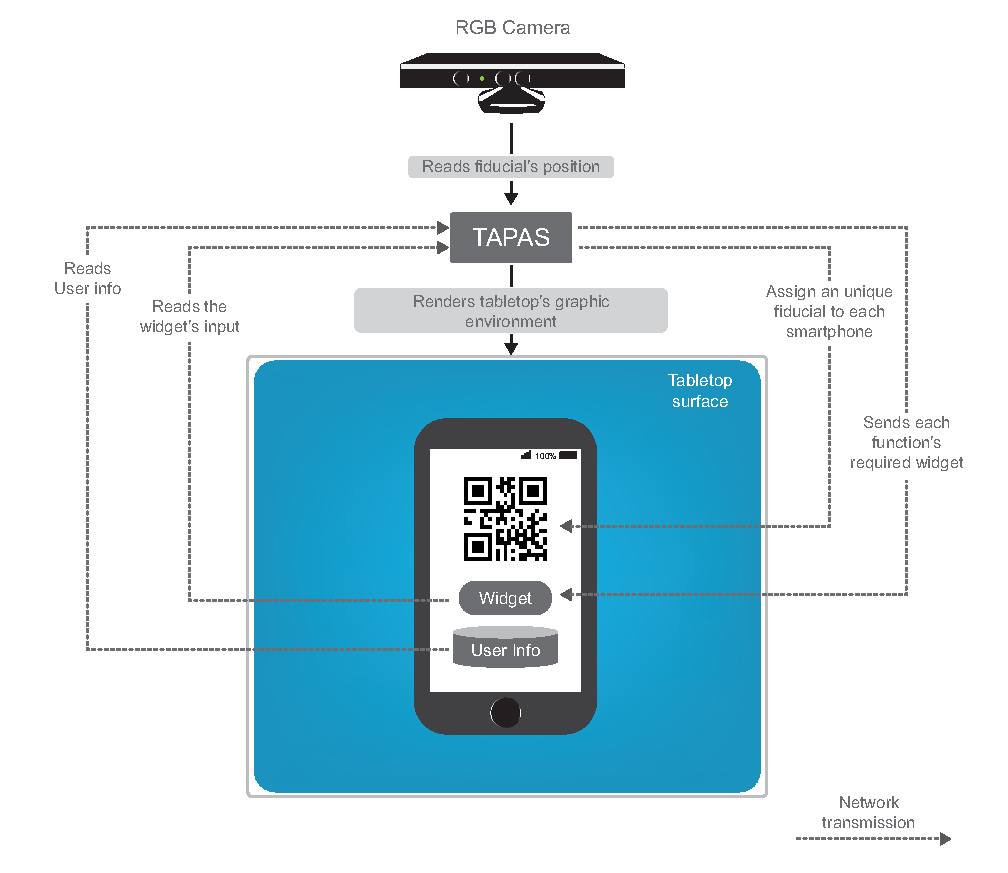
\includegraphics[width=\textwidth]{images/c4/TAPAS.eps}
\caption{The architecture of \ac{TAPAS}: using a fiducial marker --- assigned by the application itself --- and an RGB camera, \ac{TAPAS} can track a smartphone's movements on a tabletop surface; through the smartphone, \ac{TAPAS} is able to link each and every smartphone's movements to its users and display a corresponding dynamic widget.}\label{fig:arch}
\end{figure}

\subsubsection{\ac{TUIReO}}
As stated before, \ac{TAPAS} supports the \ac{TUIO} protocol and extends it to provide developers with a framework --- called \ac{TUIReO} --- that allows them to easily experiment with tracking generic programmable objects on a big display. Applications developed with this framework should foster new interactive experiences, featuring \ac{EUD} with ubiquitous tangibles with advanced feedback and input mechanisms.

The \ac{TUIO} protocol, as Kaltenbrunner et al.~\cite{kaltenbrunner2005tuio} stated, ``is an attempt to provide a general and versatile communication interface between tangible tabletop controller interfaces and underlying application layers. It was designed to meet the needs of tabletop interactive multi-touch surfaces, where the user is able to manipulate a set of objects and draw gestures onto the table surface with the fingertips.''

The \ac{TUIReO} framework (figure~\ref{fig:tuireo}) was designed to provide further interaction capabilities for multi-device environments on top of the \ac{TUIO} protocol. This allowed experimenting further with \ac{TAPAS} and block-oriented programmable objects, as reported in the next chapter.

\begin{figure}[ht!]
\centering
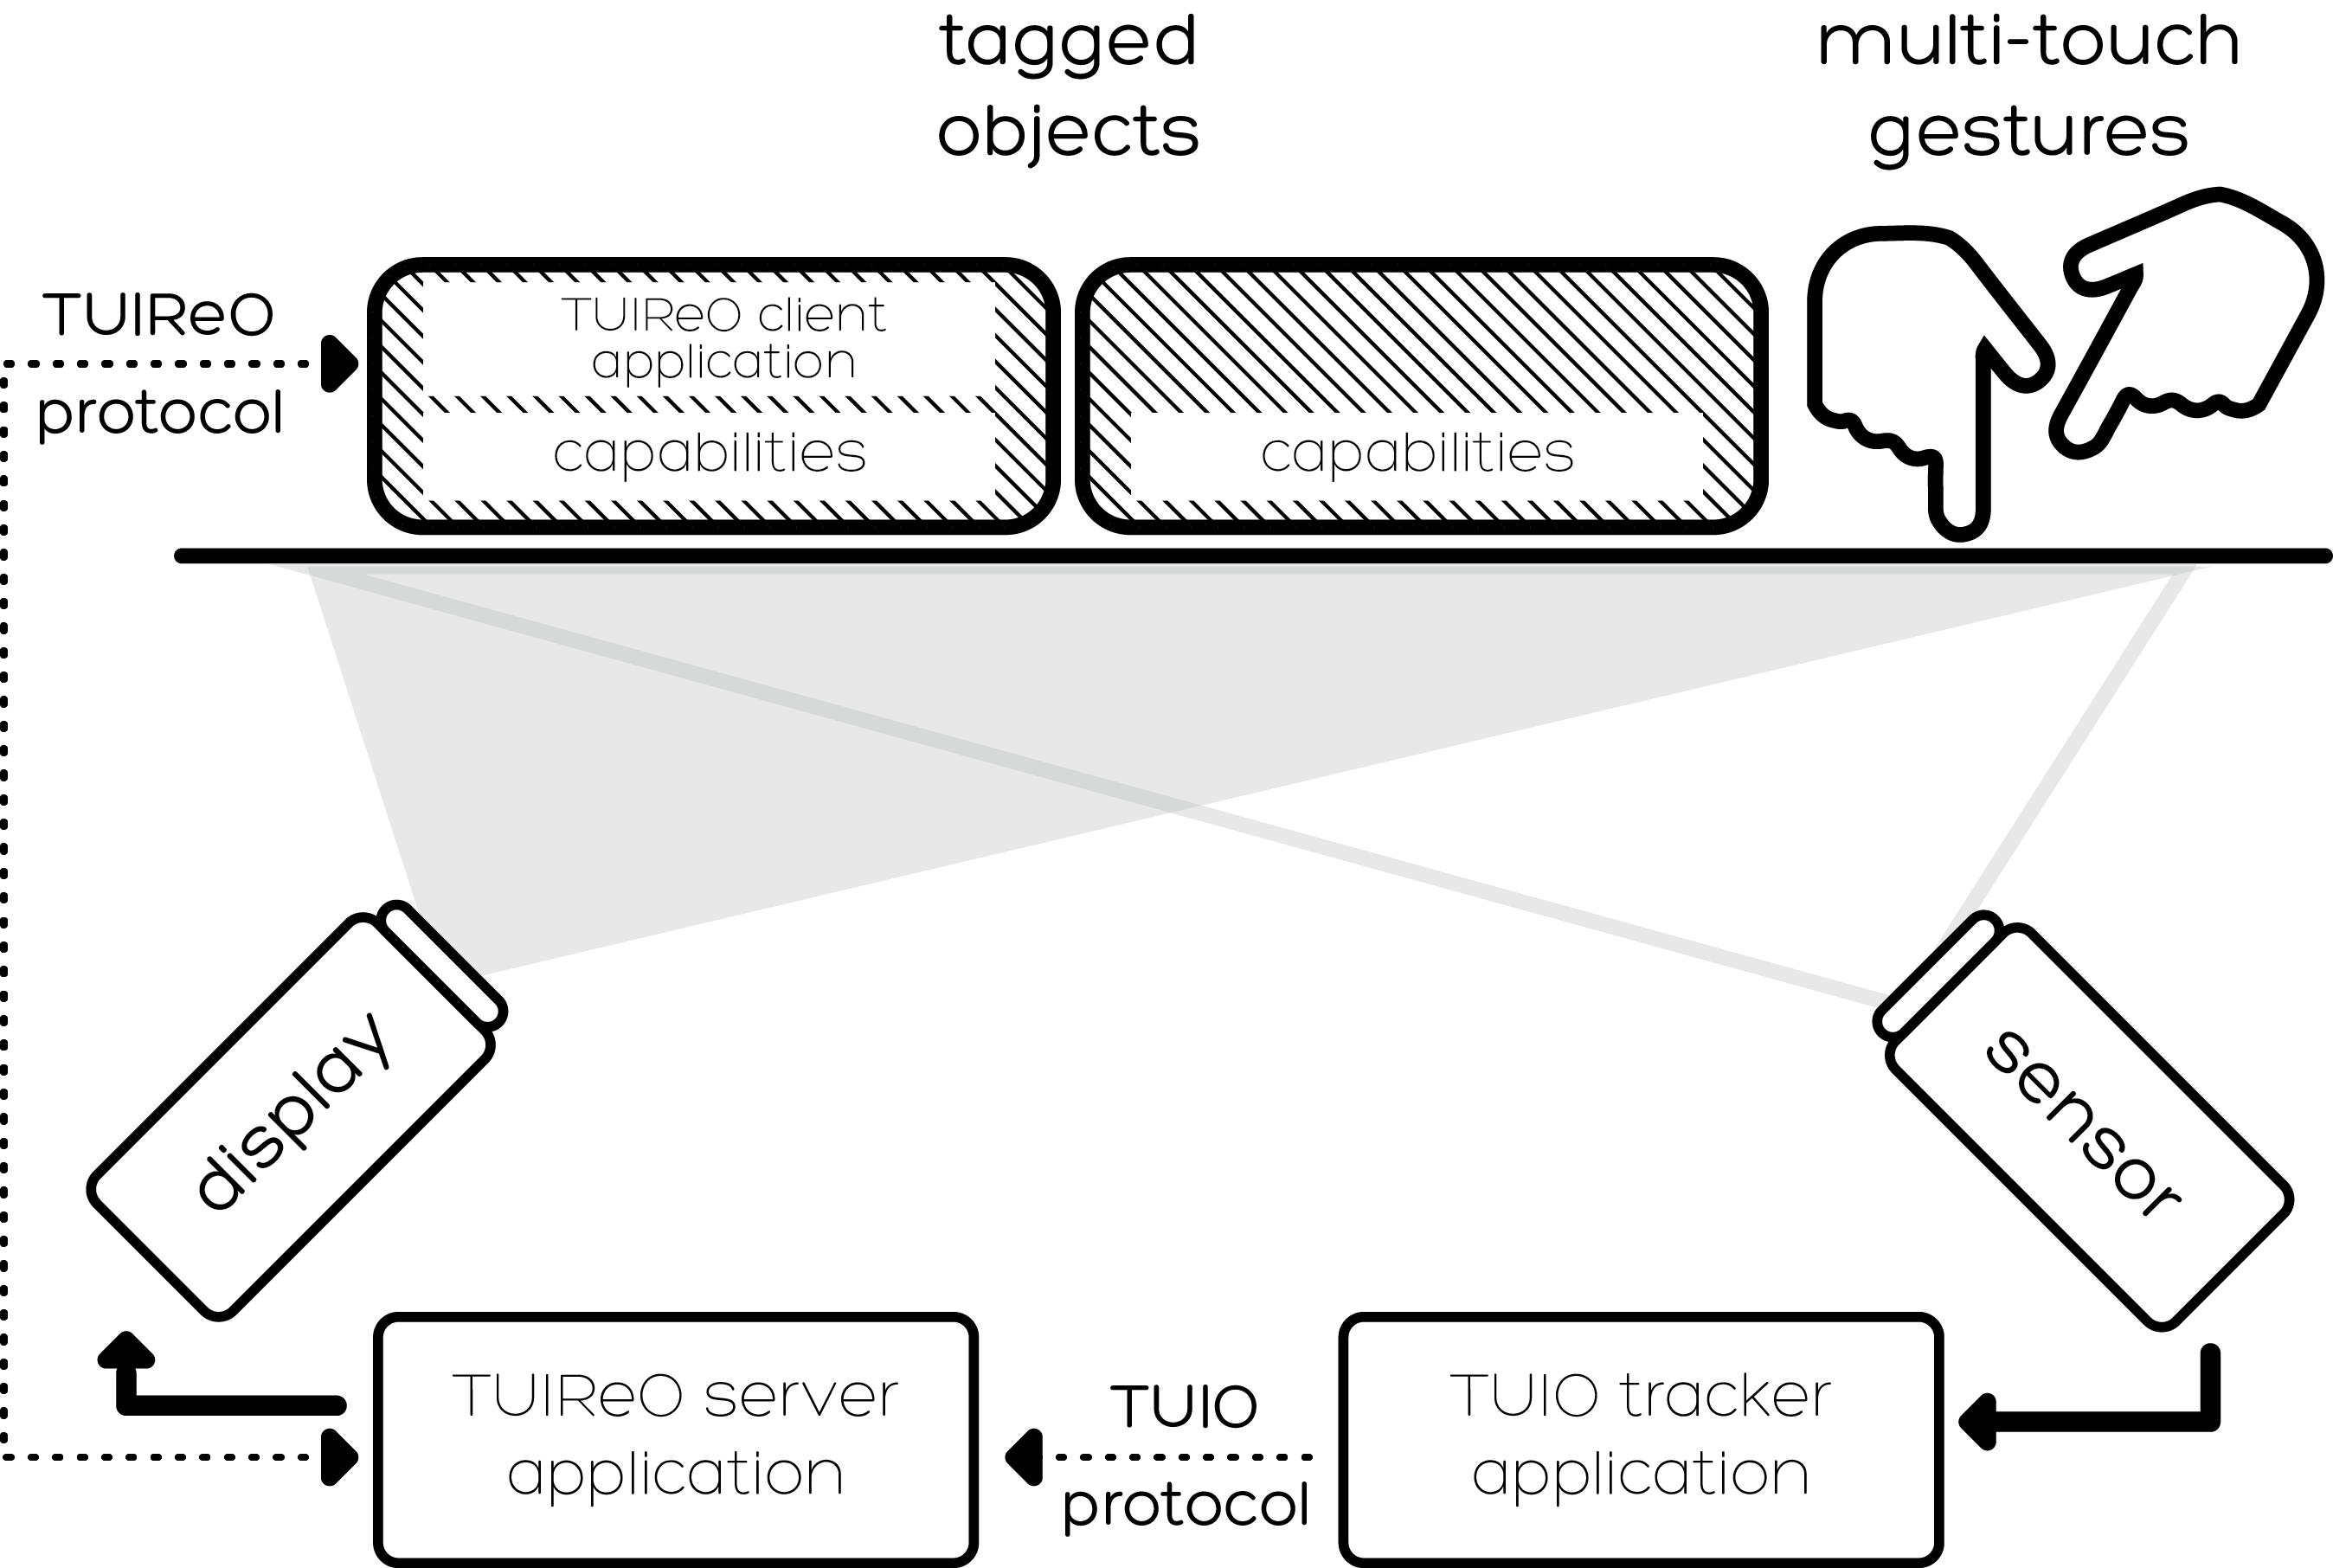
\includegraphics[width=\textwidth]{images/c4/TUIReO.png}
\caption{\ac{TUIReO} Framework Architecture}\label{fig:tuireo}
\end{figure}

\ac{TUIReO} is built on top of \ac{TUIO} to provide an abstraction layer over the capabilities of the tagged smart objects that are already handled by \ac{TUIO}. It aims to encapsulate the capabilities of a smart object --- namely the properties that the physical object offers to the environment and that can be controlled and detected remotely --- with its virtual \ac{TUIO} representation. This enables developers to fully exploit the object features, such as the inputs and outputs channels that it might provide, either physical or digital (in the form of a display or a physical button). 

Programmable objects support the following capabilities:
\begin{description}
\item[Interaction capabilities] i.e.\ buttons, multi-touch events, mid-air gestures.
\item[Display capabilities] i.e.\ LEDs, screens.
\item[Retrieval capabilities] i.e.\ storage, user's details (e.g., Facebook account).
\item[Affordance capabilities] i.e.\ shape, haptic.
\end{description}

The \ac{TUIReO} environment comprises of
\begin{enumerate*}[label=(\arabic*)]
  \item a sensor used by the \ac{TUIO} component to track tagged objects and multi-touch gestures happening over the tabletop surface, whose positions are transmitted to
  \item a display running the \ac{TUIReO} server application. The server application implements a TUIO client and stores each object’s movements and smart capabilities together, controlling the display output of the tabletop and the inputs and outputs of every object through the \ac{TUIReO} protocol.
\end{enumerate*}

\ac{TUIReO} can be considered a framework for tracking programmable objects on a tabletop and managing their physical and digital properties. It\added{s design stems from lessons learned from the development of the initial prototype reported in section \ref{sec:pdesign}; it }has been employed in \ac{TAPAS} to implement a \added{tangible }Block-based programming environment\deleted[comment={D24}]{ with the aim of fostering \ac{CT} skills}\added[comment={D25}]{, while a future evaluation needs to be carried out from a development point of view}.

\subsection{Implementation}
\added[comment={MP7}]{\ac{TAPAS} has been implemented in the form of two applications running side by side, in a client-server fashion. The first, named \ac{SPRITS}, implements the \ac{TUIReO} server application, tracking objects and gestures over a horizontal display. It is developed in C++ and sports an abstraction layer over different depth-cameras (supporting OpenNI-based}~\cite{OPENNI} \added{sensors at first) and communication protocols (\ac{TUIO} being the default one). It can be calibrated to fit any surface size (at a maximum of 2 meters distance) that the camera is pointed at.}

\added{\ac{SPRITS} tracks fiducials and touches issues to the display and streams them on the network through the \ac{TUIReO} protocol. This feed is picked up by the main \ac{TAPAS} application: it is developed in JavaScript and runs on the Web. It can run on any PC with a JavaScript-enabled browser, and can be customised using a mix of CSS (to personalise the look and feel of the displayed objects) and JavaScript (to customize the behaviour of each block).}

\section{Discussion and Post-Hoc Analysis}
The results of the study prompt to address the Research Question set out to be investigated in the introduction.

While this indeed was just a preliminary study on a specific application domain, its findings can certainly be used to highlight some of the advantages and issues with \ac{TAPAS}. \replaced[comment={D26}]{There are initial hints of it being able to support peer-to-peer collaboration (i.e.\ where all participants have the same role within the group), however it also features chaired modalities by leveraging on the use of smartphones (as suggested in~\cite{Clinch:2013uj})}{Supporting collaboration is definitely one of its major features, both peer-to-peer --- that is where all participants have the same role within the group --- and chaired modes; discovering user roles is the cornerstone, and the use of smartphones can definitely come in handy for it~\cite{Clinch:2013uj}}. Moreover, \ac{TAPAS} supports users in individual activities as well, enabling them to use their preferred tools while carefully considering the resulting privacy issues; indeed, the choice of employing smartphones as tangible probes in \acs{TAPAS} was influenced by privacy concerns, allowing it to draw upon user data while keeping the user in control of what she wants to share and with whom. For this reason, further developments are currently in the works on \acs{TAPAS}' Web app in order to develop a more sophisticated interface that enables users to effectively tweak their privacy settings and control which data \acs{TAPAS} can have access to.

The proposed interaction modality has been positively received by both end-users and domain experts, paving the way for its application in a wide range of domains where users need to perform simple tasks, either individually or collaboratively, while fostering their \ac{CT} skills. While this last point will be discussed more in details in the next chapter, \ac{TAPAS} \replaced[comment={D27}]{was successfully}{already proved to be a flexible software platform that can be easily} to a given \ac{IL} scenario by developing a set of specific functions, which can be easily assembled by users into different workflows and interact with it.

Two relevant challenges of fostering \ac{CT} skills with Tangible Programming in \ac{IL} scenarios can be identified from the findings\replaced[comment={D28}]{, one stemming from the results of \ac{TAPAS}' evaluation with end-users and another from the interviews with domain experts}{: the first stems from the results of \ac{TAPAS}' evaluation with end-users and is about the duality of composing workflows and executing workflows in tangible environments; the second challenge has emerged during the interviews with domain experts and is related to the use of Visual Languages in the domain of Tangible Programming}. 

\replaced[comment={D28}]{Firstly, t}{T}he user experience seems to differ when the tangible interaction is used for composing services with blocks (positive experience) from when users interact and collaborate on the results of the workflow execution through their smartphones (less positive experience). This could be due to the different set of constructs involved within each stage:
\begin{enumerate}
  \item Building a workflow requires the user to deal with abstract concepts --- like functions and constraints --- that are not naturally coupled with any existing physical counterpart; providing users with an intuitive visual metaphor and enabling them to interact with the system in a natural way (through a tangible) might be an effective strategy to help them build the right mental model, together with exposing the right transparency level of the workflows' inner logic in order to improve abstraction and decomposition skills, indeed helping to develop their \ac{CT} abilities.
  \item In an \ac{NUI} based environment, direct manipulation of contents is more intuitive than using intermediate control mechanisms; hence, when it comes to manipulating results produced by their workflows, users require the interface to be completely transparent, without any syntactical --- least of all tangible --- artefact to operate on an environment's constructs. 
\end{enumerate}

This contrast is also evident from the literature (see section~\ref{sec:tp}) highlighting the many differences between the \ac{PbD} and \ac{PbI} paradigms: due to its very nature, in a \ac{PbD} system the composition and execution environments are perfectly overlapped, i.e.\ the same artefacts the users operate on to program the system is used also to interact with its results; in Robot Programming by Demonstration, for instance, users teach movements to a robot by simply simulating them directly onto its body. This is radically different from a \ac{PbI} approach, where the two environments --- composition and execution --- are generally detached from one another, each one using different metaphors and concepts, e.g., the visual editor of the now-defunct Yahoo! Pipes~\cite{Pruett:2007:YP:1407887} is used to compose a pipe (data-flow) that generates a specific execution environment made of \ac{GUI} elements as designed by the user. While this distinction might be overlooked from an interaction perspective when a system only relies on a \ac{GUI}, it becomes more relevant when it is about \acp{TUI}. Even though \ac{PbI} seemed the right paradigm to choose in the analysed scenario due to its generalizability and the benefits brought to \ac{CT} skills, choosing the right paradigm according to the naturalness of interaction is arguably scenario-dependent, as is often the case with Domain Specific Visual Languages.

\replaced[comment={D28}]{Secondly, f}{F}rom the study with designers, an interesting challenge has emerged which is related to the use of Visual Languages with \acp{TUI}. In particular, the majority of examples found in the literature (section~\ref{sec:tp}) --- including \ac{TAPAS} --- use Visual Languages when employing a \ac{PbI} paradigm. 

Visual Languages have been widely used within the field of \ac{EUD} in order to ease the development process for end-users; the interaction paradigm used for Visual Languages is \ac{GUI}-based, whilst due to the selected scenario a more natural way of allowing \ac{EUD} would be to support tangible interaction. Studying whether there is an appropriate \ac{EUD} paradigm for \ac{TUI} environments requires understanding whether any of the available paradigms, e.g., \ac{PbI} and \ac{PbD}, are suitable for Tangible Programming or if, on the contrary, new paradigms need to be introduced. There is some evidence, as in Robot Programming by Demonstration for instance, that \ac{PbD} is suitable for that specific scenario using Tangible Programming but, as often happens in the \ac{EUD} community, the solution might be domain dependent.

\added[comment={D29}]{Finally, as for the preliminary studies just described, \ac{TAPAS} can support future evaluations over the effects of a tangible \ac{PbI} paradigm in relation with \ac{CT} in different \ac{IL} domains, as further reported in the next chapter.}

\section{Threats to Validity}
Here are the validity threats to the design of this study.

\paragraph{Internal Validity} The limited number of components developed and deployed to the \replaced[comment={D30}]{tested system could have influenced its usage}{system prevented from fully evaluating its usage in a real in-the-wild scenario}, thus the findings cannot be properly generalized for many other contexts. Yet, since \acs{TAPAS} was employed as a provotype --- that is to challenge users by exposing tensions and thus to support design explorations~\cite{Boer:2012ku} --- observations related to the interactions users and designers carried out can give a good insight into its real usage. The experimenter effect is concerned with any biasing effects in a study that is due to the actions of the researcher. The researcher attempted to carry out the study as objectively and as accurately as possible without interfering, acting as an observer limited to recording feedback. The subject effect could have determined changes in the participants' behaviour due to being in the study and under observation; in this case, the study was carried out within a traditional university environment with the actual group members participating to the activity.

\paragraph{External Validity} The results of the study can be generalized only in the context of the scenario where \ac{TAPAS} was deployed, although it represents quite a common setting. In order to generalize the findings to other scenarios, replication studies are needed.

\section{Contributions}
Parts of the work and results described in this chapter have been previously published in\added[comment={MP6}]{ the following}:
\begin{itemize}
  \item \added{The Literature Review described in section \ref{sec:tp} and the First Phase of the Evaluation in section \ref{sec:ev4} have been published in}~\cite{Turchi:2015dr}.
  \item \added{The Evaluation described in section \ref{sec:ev4} has been published in}~\cite{Turchi:2015kr}.
  \item \added{The Preliminary Study described in section \ref{sec:pstudy} and the Evaluation in section \ref{sec:ev4} have been published in}~\cite{turchi2017tapas}.
  \item \added{The \ac{TUIReO} Framework described in section \ref{sec:tapasarch} has been published in}~\cite{malizia2017block}.
  \item \added{The \ac{TAPAS} Architecture described in section \ref{sec:tapas} has been published in}~\cite{desolda2018tangible}.
  \item \added{The Preliminary Design of \ac{TAPAS} described in section \ref{sec:pdesign} and the Second Phase of the Evaluation in section \ref{sec:ev4} have been published in}~\cite{dix2016rich}.
\end{itemize}

\section{Conclusion}
This chapter introduced \acs{TAPAS}, an application running on a tabletop system, which allows users to develop simple workflows using their smartphones by combining a tangible and visual interaction. Its architecture and design rationale stem from a two-phases evaluation carried out with the aim of studying the effects of physical manipulation in \ac{IL} domains on the development of \ac{CT} skills.

From the first phase of the study (involving second-year undergraduates working in groups) it seems that \ac{TAPAS} provides a positive user experience and could be used in \ac{IL} scenarios where learning is self-directed and driven by people's preferences and intentions during their daily activities; a potential side effect caused by employing it to support learning might be a development of \ac{CT} skills, thanks to its design rationale, which will be discussed and further evaluated in the next chapter.

However, from the findings, it also appears that coupling tangible interaction with a \ac{PbI} paradigm causes an incompatibility of interaction styles between the composition and the execution environments, where the use of a different tangible-based syntactic construct in the former causes the need for a different interaction style to be used in the latter.

The second phase of the study was focused on its interaction modality and involved a group of interaction design experts; the results show that \replaced[comment={D32}]{the system design presents positive elements to support collaboration in \ac{IL} domains}{participants liked the proposed interaction style}, recognizing the potential of the exploited puzzle metaphor in allowing end-users to develop simple workflows. They also suggested extending the platform in order to cope with more complex data to be manipulated by users. However, \replaced[comment={D31, DC33}]{it was also pointed out that employing a Visual Language in a \ac{TUI} system doesn't always provide}{from the results it seems that exploiting Visual Languages within a \ac{TUI} system might not be the best way of providing} users with a natural interaction experience, thus further investigations are needed to determine the role of the scenario in the choice of the right paradigm (i.e.\ \ac{PbI} vs \ac{PbD}).

In the next chapter, the main Research Question of this thesis will be laid down in combination with gameplay activities and \ac{TAPAS} will be employed to test the related hypothesis.